\documentclass[a4paper]{scrartcl}
\usepackage{palatino}
%\usepackage{url}
%\usepackage{xcolor}
%\usepackage[colorlinks=true, linkcolor=black, linkbordercolor=blue, urlbordercolor=blue, urlcolor=black, pdfborderstyle={/S/U/W .5}]{hyperref}
%\usepackage{breakurl}
\usepackage{graphicx}
%\usepackage{multirow}
\usepackage{fancyhdr}
%\usepackage{comment}
%\usepackage{printlen} % Print lengths using specified units. 
\usepackage[pdfborder=0 0 0]{hyperref}
%\usepackage{booktabs}
\usepackage[utf8]{inputenc} % Umlaute üöä auch normal benutzen und nicht maskieren
%\usepackage[rightcaption]{sidecap}  % caption beside figure
\usepackage{amsmath, amssymb}
\usepackage{listings}
%\usepackage{subfigure}
%\usepackage{setspace}
\usepackage{threeparttable}
\usepackage{tabularx}
%\usepackage{todonotes}
\usepackage{paralist}
%\usepackage{siunitx}
\usepackage{amsfonts}
\newcommand{\tickYes}{\checkmark}
\usepackage{pifont}
\newcommand{\tickNo}{\hspace{1pt}\ding{55}}
\usepackage{xspace}
\usepackage{dirtree}

%\usepackage[width=.75\textwidth]{caption}

\usepackage{color}
\definecolor{gray}{rgb}{0.4,0.4,0.4}
\definecolor{darkblue}{rgb}{0.0,0.0,0.6}
\definecolor{cyan}{rgb}{0.0,0.6,0.6}


% custom commands
\newcommand{\wik}{\textit{Wiktionary}\xspace}
% http://www.ctan.org/tex-archive/fonts/ps-type1/cm-super/
\usepackage[T1]{fontenc} % use high quality fonts, please install cm-super
\newcommand{\lemon}{\emph{lemon} }
\newcommand{\lemonnospace}{\emph{lemon}}
\newcommand{\footnoteUrl}[1]{\footnote{\url{#1}}}

%%%% LISTINGS
\usepackage{listings} % Typeset source code listings using LaTeX.
% listing styles
\lstset{
    numberbychapter=false,
    numbers=left,
    numberstyle=\tiny,
    basicstyle=\ttfamily\fontsize{8}{8}\selectfont,
%    tabsize=2,
%    framexleftmargin=2pt,
    captionpos=b,
    frame=single,
    breaklines=true,
    columns=fullflexible,
    showstringspaces=false,
    commentstyle=\color{gray},
    literate={ö}{{\"o}}1
               {ä}{{\"a}}1
               {ü}{{\"u}}1
}
%\lstdefinestyle{rdf}{numberblanklines=true, morekeywords={}}
\lstdefinestyle{sparql}{numberblanklines=true, morekeywords={SELECT, FROM, WHERE, FILTER, GROUP BY, IN, AS, LIMIT, OFFSET, PREFIX, OPTIONAL, UNION}}
\lstdefinestyle{N3}{numberblanklines=true, morekeywords={foaf, prefix, rdf, skos, rdfs, ex, xsd, wr, wt, dc, lemon, doap, @prefix}}
\lstdefinestyle{wikitext}{numberblanklines=true, morekeywords={\{\{, \}\}, =, |, [[, ]]}}
%\usepackage{textcomp}
\lstdefinestyle{XML}
{
  morestring=[b]",
  morestring=[s]{>}{<},
  morecomment=[s]{<?}{?>},
  stringstyle=\color{black},
  identifierstyle=\color{darkblue},
  keywordstyle=\color{cyan},
  morekeywords={xmlns,version,type}% list your attributes here
}
%%%% todo
% \newcommand{\todo}[1]{\textbf{[ToDo: #1]}}
% draws PDF notes instead of in-text todos
%\usepackage{pdfmarginpar}\newcommand{\todo}[1]{\pdfmarginpar[Note]{ToDo: #1}}
%\newcommand{\todo}[1]{}

\hypersetup{colorlinks=true,urlcolor=blue,linkcolor=black,citecolor=black}

%resize texttt (doesnt play well with palatino I guess )
%\let\Oldtexttt\texttt
%\renewcommand{\texttt}{\small\Oldtexttt}

\newcommand{\NAME}{Flexible RDF data extraction from Wiktionary}

\newcommand{\TITLE}{\NAME}
\newcommand{\TITLER}{Leveraging the power of community build linguistic Wikis}
\newcommand{\KEYWORDS}{Semantic Web, Natural Language Processing, Information Extraction}

\pdfinfo{
	/Title (\TITLE)
	/Creator (TeX)
	/Keywords (\KEYWORDS)
	/Producer (pdfTeX and Document $Revision: 5900 $)
	/Author (Jonas Brekle)
	%/CreationDate (D:19980212201000)
	%/ModDate (D:19980212201000)
	/Subject (\NAME)
}

\graphicspath{{images/}} % include-pfad für Grafiken
\DeclareGraphicsExtensions{.pdf,.png}


% \renewcommand{\vec}[1]{\overrightarrow{#1}}

\fancyhf{}
\pagestyle{fancy}
% Seitenzahl bei geraden/linken Seiten nach links/aussen
\fancyhead[R]{\thepage}

\fancyhead[L]{\leftmark}% Kapitel/Abschnitt



\begin{document}

\begin{titlepage}
\vspace{2 cm}
\thispagestyle{empty}
\begin{center}
\Large{
Universität Leipzig\\
Fakultät für Mathematik und Informatik\\
Institut für Informatik\\
}
\vspace{3 cm}
\textbf{
	\Large{
	\TITLE\\
	}
}

\TITLER\\
\vspace{2 cm}
Masterarbeit\\
im Studiengang Master Informatik

\end{center}
\vspace{6 cm}

\begin{flushleft}
\begin{tabular}{lll}
& & \\
\textbf{eingereicht von:} & & Jonas Brekle\\
& & \\
& & \\
\textbf{eingereicht am:} & & 1. August 2012\\
& & \\
& & \\
\textbf{betreuender Professor:} & & Prof. Dr. Ing. habil. Klaus-Peter Fähnrich\\
& & \\
& & \\
\textbf{Betreuer:} & & Dipl. Inf. Sebastian Hellmann
\end{tabular}
\end{flushleft}
\end{titlepage}

\thispagestyle{empty}
\begin{abstract}
We present a declarative approach implemented in a comprehensive open-source framework (based on \textit{\mbox{DBpedia}}) to extract lexical-semantic resources (an ontology about language use) from \wik. 
The data currently includes language, part of speech, senses, definitions, synonyms, taxonomies (hyponyms, hyperonyms, synonyms, antonyms) and translations for each lexical word.
Main focus is on flexibility to the loose schema and configurability towards differing language-editions of \wik.
This is achieved by a declarative mediator/wrapper approach.
The goal is to allow the addition of languages just by configuration without the need of programming, thus enabling the swift and resource-conserving adaption of wrappers by domain experts. 
%TODO maybe add crowd sourcing and DBpedia againcd 
%to new usage scenarios by crowd-sourcing ( proven working by DBpedia \cite{dbpedia_jws_09} and the \textit{Mappings Wiki}\footnote{a community interested in curating the DBpedia dataset collaboratively maintains the core of the extraction configuration --- the infobox label mappings --- at \url{http://mappings.dbpedia.org/}}).
The extracted data is as fine granular as the source data in \wik and additionally follows the \textit{lemon} model. 
It enables use cases like disambiguation or machine translation. 
By offering a linked data service, we hope to extend DBpedia's central role in the LOD infrastructure to the world of Open Linguistics.
\end{abstract}

\vfill
I thank Sebastian Hellmann for the courageous supervision and a professional research environment; furthermore Theresa for her support. Without them, this work would not have been possible.
\pagebreak

\pagenumbering{Roman}
\setcounter{page}{1}

% Inhaltsverzeichnis
\tableofcontents
\pagebreak

%changing the pagenumbering style (roman->arabic) resets pagecoutner. workaround:
\newcounter{tmppage}
\setcounter{tmppage}{\value{page}}
\pagenumbering{arabic}
\setcounter{page}{\value{tmppage}}

\section{Introduction}

\subsection{Motivation}

The topic of this thesis will be the flexible extraction of semantically rich data from \wik.
The resulting data set is a lexical resource for computer linguistics.
But however the focus is not on linguistics but on data integration: information extraction from wikis can be conducted in two ways --- in perspective of 1) text mining, where the wiki is seen as a corpus or 2) interpreting the wiki as a collection of semi-structured documents.
The latter is the way we will see it and how DBpedia was designed as it enables the definition of \textit{extractors}, that interpret wiki pages.
Also opposed to text mining, DBpedia allows to tailor the extracted data step by step closer to the intended semantic of the wikitext.
Additionally weak signals (facts that don't have much support, that are only stated once) can be taken account of.
DBpedia creates an ontology from Wikipedia, that is roughly said, a database of world knowledge.
Opposed to Wikipedia, the DBpedia knowledge base can be queried like a database, comibining information from multiple articles.
To conduct a analogous transformation on \wik, we analysed the major differences and found that \wik is on one hand richer in structured informationbut also  this structure varies widely.
So we propose an declarative framework, built on top of DBpedia, to convert \wik into a linguistic ontology about languages, about the use of words, about their properties and relations.
We will show which unique properties such a knowledge base has and what possible applications are.
The declarative extraction rules can be maintained by a community of domain experts, that don't necessarily need programming skills.
As will be shown, this is crucial for the approach to succeed on a long term.
DBpedia has proven such a approach to be working and scaling.
The goal of DBpedia is to provide a tool for unsupervised but highly configurable ontology construction.
By using and extending DBpedia \wik can be automatically transformed into a machine readable dictionary --- with substantial quantity and quality.

\subsection{Problem}
\label{intro}
%Why is it important
The exploitation of community-built lexical resources has been discussed repeatedly.
\wik is one of the biggest collaboratively created lexical-semantic and linguistic resources available, written in 171 languages (of which approximately 147 can be considered active\footnote{\url{http://s23.org/wikistats/wiktionaries_html.php}}), containing information about hundreds of spoken and even ancient languages. 
For example, the English \wik contains nearly 3 million words\footnote{See \url{http://en.wiktionary.org/wiki/semantic} for a simple example page}.
A \wik page provides for a lexical word a hierarchical disambiguation to its language, part of speech, sometimes etymologies and most prominently senses.
Within this tree numerous kinds of linguistic properties are given, including synonyms, hyponyms, hyperonyms, example sentences, links to Wikipedia and many more.
\cite{meyer_2011b} gave a comprehensive overview on why this dataset is so promising and how the extracted data can be automatically enriched and consolidated. 
Aside from building an upper-level ontology, one can use the data to improve NLP solutions, using it as comprehensive background knowledge.
The noise should be lower when compared to other automatic generated text copora (e.g. by web crawling) as all information in \wik is entered and curated by humans.
Opposed to expert-built resources, the openness attracts a huge number of editors and thus enables a faster adaption to changes within the language.

%What's the problem?
The fast changing nature together with the fragmentation of the project into  \wik language editions (\textit{WLE}) with independent layout rules (ELE) poses the biggest problem to the automated transformation into a structured knowledge base.
We identified this as a serious problem:
Although the value of \wik is known and usage scenarios are obvious, only some rudimentary tools exist to extract data from it.
Either they focus on a specific subset of the data or they only cover one or two WLE.
The development of a flexible and powerful tool is challenging to be accommodated in a mature software architecture and has been neglected in the past.
Existing tools can be seen as adapters to single WLE --- they are hard to maintain and there are too many languages, that constantly change. 
Each change in the \wik layout requires a programmer to refactor complex code. 
The last years showed, that only a fraction of the available data is extracted and there is no comprehensive RDF dataset available yet. 
The key question is: 
Can the lessons learned by the successful DBpedia project be applied to \wik, although it is fundamentally different from Wikipedia? 
The critical difference is that only word forms are formatted in infobox-like structures (e.g. tables).
Most information is formatted covering the complete page with custom headings and often lists. 
Even the infoboxes itself are not easily extractable by default DBpedia mechanisms, because in contrast to DBpedias \textit{one entity per page} paradigm, \wik pages contain information about \textit{several} entities forming a complex graph, i.e. the pages describe the lexical word, which occurs in several languages with different senses per part of speech and most properties are defined \textit{in context} of such child entities.
%A page describes a word, but for example senses are distinct entities, and most properties are defined \textit{in context} of such child entities.
%How do we solve it?
Opposed to the currently employed classic and straight-forward approach (implementing software adapters for scraping), we propose a declarative mediator/wrapper pattern. 
The aim is to enable non-programmers (the community of adopters and domain experts) to tailor and maintain the WLE wrappers themselves. 
We created a simple XML dialect to encode the ``entry layout explained'' (ELE) guidelines and declare triple patterns, that define how the resulting RDF should be built. 
This configuration is interpreted and run against \wik dumps. 
The resulting dataset is open in every aspect and hosted as linked data\footnote{\url{http://wiktionary.dbpedia.org/}}. 
Furthermore the presented approach can be extended easily to interpret (or \textit{triplify}) other MediaWiki installations or even general document collections, if they follow a global layout.


In section~\ref{sec:basics} I will introduce the domain of information extraction from wikis and RDF and related concepts, that form the basis of this thesis.\\
In section~\ref{sec:problem} and \ref{sec:specification} I give an overview on  requirements of the developed software, that arise in context of the DBpedia project and explain resulting specifications.\\
In the following section~\ref{sec:implementation} I will present some implementation details, that turned out to be essential for the success of of the approach. Finally in section~\ref{sec:evaluation} the created dataset is evaluated and compared with existing datasets. The thesis is written in a top-down manner, so when ever questions seem to remain open, continue reading, as details will follow later.

\newpage


\section{Background}
\label{sec:basics}

In the following a short overview on underlying technologies is given. 

\begin{figure}
  \centering
    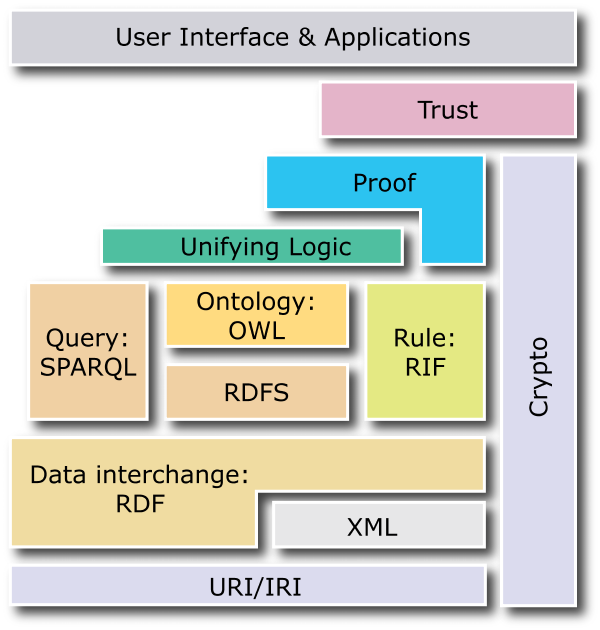
\includegraphics[width=0.5\textwidth]{layerCake.png}
  \caption{Semantic Web Technologien}
  \label{fig:layercake}
\end{figure}

\subsection{Semantic Web}

The world wide web is one the most important inventions of our time. 
It enables the global access to documents and real time communication between individuals.
This achieved by an interoperable infrastructure of independent networks, that can route any communication between two points.
From our current perspective on the last three decades, this even seems technologically simple and maintainable at a reasonable cost.
Furthermore the resulting benefits to our economy and society are beyond all expectations. A hole new industry was created and most industries are substantially influenced in their processes.
The costs of communications dropped and public and private communications alike switched mostly to the new medium.
The world wide web is enabled by a set of related technologies, which can be summarized to the following core concepts:
\begin{itemize}
\item TCP/IP addressing, transmission and routing
\item client/server communication protocols like HTTP
\item interlinked documents containing data (e.g. XML) or services (or interactive content) valuable for humans
\end{itemize}
While these technologies are well established and scale up to a huge amount of data, the users --- humans --- can barely cope with this amount of data offered. 
If one considers the WWW a information system, it only offers basic retrieval methods and most critical, it is fragmented into heterogeneous subsystems (which however can offer very good retrieval methods). 
But global interoperability is not supported on content level. Data is controlled by applications, and each application keeps it to itself\footnoteUrl{http://www.w3.org/2001/sw/}.
From a perspective of data integration, semantics are often vague or undefined. It is often unclear which entity a document refers to. Documents are only interlinked by untyped relations. These are strong limitations: if the data is too much for a human to read and machines do not have deeper insight into it, the dataset as a whole can be seen as inaccessible. Of course the way the WWW works today seems to be well suited. Programmable Webservers e.g. with PHP made the web interactive, enabling social interaction or collaborative editing. But still future development is blocked by the human-centric nature of the web. If all the knowledge humanity acquired and wrote down in e.g. Wikipedia would be also available to information systems in a structured way, even more knowledge could be inferred automatically and e.g. artificial intelligence, expert systems or search would be boosted dramatically. The key to solving this issue lies (according to \cite{berners}) in the establishment of \textit{Linked Data} (which will be explained in the next section). The use of machine readable data and annotation of text with such data is crucial for information technology to enter the next level.
So to conclude: the problem is the amount of knowledge, and the lack of formalization e.g. machine readability. Even data that is already structured often lacks a defined semantic or the semantic is not formalized. The web as we know it is a web of documents, the target is the web of data. Instead of just documents linking to each other, instances should be globally interlinked. Consider this example: A company stores costumer information about you in its relational database; facebook keeps record of your activities in their distributed database and you yourself have a blog on your own webserver. Why shouldn't all this personal information be linked\footnote{The reader may object privacy issues; but the focus of this thesis is on data integration. These two topic have to be considered separately: just because data is interoperable, it is not accessible. Even more: if you avoid redundancy, you gain control over your data. How this control can be achieved is topic to current research but already very promising. Cf. WebID}? By a global identifier for \textit{you}. Why do we have to supply contact information over and over again, although its database 101 that redundancy is bad. The answer is incompatibility on many levels. The ideal would be that all data is interoperable by design. Shortly after the invention of concepts for the WWW, Tim Berners-Lee et al. came up with the Idea of the Semantic Web: an WWW where intelligent agents can act on behalf of users, to find information or communicate. They have a shared syntax and vocabulary, use ontologies as background knowledge and thus get deeper to the intended semantic of things.
The Semantic Web (SW) is a set of complementary technologies, which are depicted in figure~\ref{fig:layercake}. It is a layered model to represent, query and manage information.\\
The effort was initiated in 2001 by Tim Berners-Lee, who defined it as 
\begin{quote}
"`an extension of the current web in which information is given well-defined
meaning, better enabling computers and people to work in cooperation"'.
\cite{berners}
\end{quote}
Dies geschieht durch verschiedene Ansätze: zunächst durch das Anreichern von (u. U. semi-struk\-tur\-iert\-en) Dokumenten durch Metainformationen schon beim Erstellungsprozess (wenn zum Beispiel ein Name in einem Dokument vorkommt, kann er in einer Art und Weise markiert werden, die allen verarbeitenden Systemen durch ein gemeinsames Vokabular als "`Personen-Markierung"' bekannt ist). Für diese Annotation wird zum Beispiel RDFa\footnoteUrl{http://www.w3.org/TR/xhtml-rdfa-primer/} genutzt. Des Weiteren wird Wissen in Form von Ontologien aufbereitet, die keine unstrukturierten Informationen enthalten, sondern lediglich \emph{wahre Aussagen} in einem formellen Format. Die Nutzung eines gemeinsamen dokumentierten Vokabulars (also die Einigung auf eine Sprache) sowie die Entwicklung offener Standards soll die Verständigung garantieren. Die Einbeziehung bereits existierender Webstandards (wie URIs oder das HTTP-Protokoll) soll eine schnelle Verbreitung ermöglichen. Dadurch soll Wissen für maschinelle Verarbeitung nutzbar gemacht werden\footnote{Allerdings wird dabei ausdrücklich nicht versucht, mithilfe künstlicher Intelligenz oder heuristischer Verfahren die Semantik für die Maschine verständlich zu machen, sondern lediglich sinnvoll repräsentierbar und damit verarbeitbar.} (vgl. \cite{hitzler}).\\
Die zentrale Technologie zur Datenrepräsentation ist RDF\footnoteUrl{http://www.w3.org/RDF/}. RDF/XML\footnoteUrl{http://www.w3.org/TR/rdf-syntax-grammar/} bzw. N3\footnoteUrl{www.w3.org/DesignIssues/Notation3} sind konkrete Kodierungen von RDF, auf welche hier nicht näher eingegangen wird. SPARQL dient als Anfragesprache für RDF-Graphen (siehe Abschnitt \ref{sec:sparql}). 

\subsection{RDF}
RDF steht für Resource Description Framework. Es ist ein Datenmodell zur Beschreibung von Web-Ressourcen (nicht nur Webseiten usw., denn jedes Ding der Welt kann über eine URI identifiziert werden), welche über eine URI\footnoteUrl{http://tools.ietf.org/html/rfc3986} identifiziert werden. Eine Ressource ist dabei eine Entität, über die Aussagen der Form \textit{"`Subjekt Prädikat Objekt"'} --- ähnlich einem natürlichsprachlichen Satz --- getroffen werden können.\\
So kodiert zum Beispiel das Tripel \\
\begin{lstlisting}[style=N3]
<http://example.com/Alice> rdf:type foaf:Person
\end{lstlisting}
die Aussage ``Alice ist eine Person''. Dabei ist Folgendes zu betrachten: Auch Subjekt, Prädikat und Objekt sind URIs, werden aber optional mit Prefixen abgekürzt (deren Definition hier ausgelassen wurde); außerdem wird das FOAF Vokabular\footnoteUrl{http://xmlns.com/foaf/0.1/} genutzt. Ein Tripel wird im Kontext der Graphentheorie interpretiert: Subjekt und Objekt sind Knoten --- das Prädikat ist der ``Typ'' der Kante.\\
\begin{figure}[h]
  \centering
    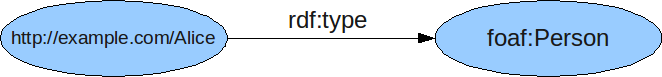
\includegraphics[width=0.5\textwidth]{triple-graph.png}
  \caption{Das Tripel als Graph}
  \label{fig:triple-graph}
\end{figure}
\\
Es entsteht (bei mehreren Tripeln) ein gerichteter Graph, der eine Ontologie repräsentiert. Graphen sind als abstraktes Konzept viel einfacher und verlässlicher zugänglich für Algorithmen als natürliche Sprache. Außerdem lassen sich implizite Informationen (zum Beispiel transitive Relationen oder geerbte Eigenschaften) ableiten oder Widersprüche finden\footnote{Access Control, Logic and Proof: \url{http://www.w3.org/2000/01/sw/#access}}.\\
Die Tatsache, dass hier kein hierarchisches Baummodell, sondern ein Graph zur Repräsentation gewählt wird, lässt sich auch damit begründen, dass Aussagen (bezüglich Beziehungen zweier Resourcen zueinander) oft nicht eindeutig einer von beiden zugeordnet werden können. Des Weiteren entspricht ein flaches Netz eher der dezentralen Struktur des Webs: Die Informationen sind verteilt und beim Zusammenführen zweier Informationsquellen stellt sich --- zumindest auf diesem Niveau --- kein Problem von Schema-Matching ein, denn das Schema ist bei allen Quellen gleichermaßen frei (vgl. \cite{hitzler}). Object-Matching soll von Beginn an vermieden werden, indem (wie oben erwähnt) ein gemeinsames Vokabular und somit überall eine eineindeutige URI für alle Objekte (Ressourcen) genutzt wird. In der Praxis besteht dieses Problem natürlich weiterhin.\\
Das Objekt eines Tripels kann in RDF auch ein Literal\footnoteUrl{http://www.w3.org/TR/rdf-concepts/#section-Graph-Literal} sein. Literale sind direkte \emph{Werte}, über die keine weiteren Aussagen getroffen werden --- also zum Beispiel Zahlen oder Zeichenketten.\\ 
Man unterscheidet zwei Arten von Literalen:
\textit{plain literals} (mit optionalem \textit{language Tag}) und \textit{typed literals}, die einen Datentyp haben, der mit einer URI angegeben wird. Im folgenden Beispiel wird das Literal mit einem selbst definierten Datentyp typisiert:

\vspace{0.2ex}

\begin{lstlisting}[style=N3]
ex:Alice foaf:birthday "22.09.1986"^^ex:germanDate
\end{lstlisting}

\subsection{Linked Data}
\textit{Linked Data} is the simplest and yet most important mechanism to retrieve RDF data: as described, entities are identified URI's. When choosing the URL's one should pick a namespace under her authority, so that she can provide \textit{some} data about that entity under that URL. As defined by W3C\footnoteUrl{http://www.w3.org/DesignIssues/LinkedData.html}, the requirements for Linked Data are as follows:

\begin{enumerate}
\item Use URIs as names for things
\item Use HTTP URIs so that people can look up those names.
\item When someone looks up an URI, provide useful information, using RDF
\item Include links to other URIs. so that they can discover more things.
\end{enumerate}
 
\begin{quotation}
The first \textit{Linked Data} principle advocates using URI references to identify, not just Web documents and digital content, but also real world objects and abstract concepts. These may include tangible things such as people, places and cars, or those that are more abstract, such as the relationship type of knowing somebody, the set of all green cars in the world, or the color green itself. This principle can be seen as extending the scope of the Web from online resources to encompass any object or concept in the world. The HTTP protocol is the Web’s universal access mechanism. In the classic Web, HTTP URIs are used to combine globally unique identification with a simple, well-understood retrieval mechanism. Thus, the second Linked Data principle advocates the use of HTTP URIs to identify objects and abstract concepts, enabling these URIs to be dereferenced (i.e., looked up) over the HTTP protocol into a description of the identified object or concept~\cite{linkeddata-book}.
\end{quotation}
The lookup of URI can even be enhanced with a mechanism called \textit{Content Negotiation}: Based on the HTTP \textit{accept} header (that is set by the application requesting), different types of formatting can be used in the response. If for example a human browses RDF data using a web browser, a HTML version of the RDF data can be generated easily. If an application requests RDF data it would set the accept header to \texttt{application/rdf+xml} and get XML, which easy to read by machines, nut not humans. The mechanism is also transparent, it happens server side at request time.  Modern RDF stores like \textit{Virtuoso} have built in support for \textit{Linked Data} with \textit{Content Negotiation}.

These four basic principles together make a fundamental difference regarding the architecture of Linked Data seen as a database. Instead of custom communication protocols, well established web standards are used. This makes it interoperable at a technical level and easy to adopt.
And it is backward compatible to very simple solutions: If one wants to publish \textit{Linked Data}, no RDF store is required at all, one could as well use a file server, with the documents available materialized.
Also \textit{Linked Data} implicitly is a \textit{basic distributed database}: Even though the query language is limited to a simple GET (for now), one can easily access data on different physical servers at no cost. Also load balancing is easy by deploying any default web proxy. Of course there if no free lunch, many topics that have been long solved on traditional relational databases, have still to be solved for RDF stores. And this little collection of advantages is not meant to compare RDF stores to relational databases, but it should show how the use of open web standards can help solving hard problems \textit{by design}. Other non-relational systems (key-value stores like Apache Cassandra or document stores like CouchDB) have shown that it is possible to make distributed databases scale and simultaneously simplify access mechanisms. RDF stores should analogously extend the expressiveness of the data model, but too be more open and designed to integrate easy.

  \begin{table}[htb]
  	\small
  	\caption{five star rating of Linked Data}
	\begin{tabular}{rp{0.7\textwidth}}
$\bigstar$ & Available on the web (whatever format) (optionally with an open licence, to be \textit{Open Data}) \\ 
$\bigstar\,\bigstar$ & Available as machine-readable structured data (e.g. excel instead of image scan of a table) \\ 
$\bigstar\,\bigstar\,\bigstar$ &  two stars plus use of a non-proprietary format (e.g. CSV instead of excel) \\ 
$\bigstar\,\bigstar\,\bigstar\,\bigstar$ & All the above plus, Use open standards from W3C (RDF and SPARQL) to identify things, so that people can point at your stuff \\ 
$\bigstar\,\bigstar\,\bigstar\,\bigstar\,\bigstar$ & All the above, plus: Link your data to other people’s data to provide context
    \end{tabular}
  \end{table}


\subsection{SPARQL}
\label{sec:sparql}
SPARQL\footnote{\url{http://www.w3.org/TR/rdf-sparql-query/} \\
bzw. \url{http://www.dajobe.org/2005/04-sparql/SPARQLreference-1.8-us.pdf}} steht für \emph{SPARQL Protocol and RDF Query Language} und ist eine Anfragesprache für RDF-Graphen sowie ein Protokoll für deren Nutzung über einen Webservice. Mit ihr können Literale, Ressourcen oder ganze Teilgraphen extrahiert werden. Sie hat sich aus anderen Sprachen, wie SquishQL\footnote{siehe \cite{squishQL}}, RDQL\footnoteUrl{http://www.w3.org/Submission/RDQL/}, RQL\footnoteUrl{http://139.91.183.30:9090/RDF/RQL/} oder SeRQL\footnote{siehe \cite{serql}} (vgl. \cite{compQL}), entwickelt und stellt nun den offiziellen Standard des W3C dar.\\
Eine kurze Übersicht\footnote{Hier werden lediglich für das weitere Verständnis zentrale Ideen erläutert --- für eine umfassende und detaillierte Beschreibung ist der Standard zu konsultieren.} über die Features der Sprache werde ich im Folgenden geben.\\
\vspace{0.1cm}\\
Es gibt 4 Typen von SPARQL Querys:
\begin{itemize}
	\item{SELECT um Daten, die auf ein angegebenes Muster passen (\emph{matchen}), zu extrahieren}
	\item{ASK um zu prüfen, \emph{ob} ein Muster im Graph existiert}
	\item{CONSTRUCT gibt einen Graph zurück, der unter Umständen durch ein Such-Muster erzeugt wurde oder explizit angegeben wird}
	\item{DESCRIBE liefert Informationen über gematchte Ressourcen (ist nicht standardisiert, abhängig von der Konfiguration der Datenbank, oft beschreibende Eigenschaften, wenn diese eingetragen wurden)}
\end{itemize}
Eine SPARQL-Anfrage (Query) lässt sich in folgende Teile aufgliedern:
\begin{itemize}
	\item{Prolog\\um Prefixe und Base-URI zu deklarieren. Relative URIs, die innerhalb des Querys vorkommen, werden auf die Base-URI bezogen. Prefixe sind Abkürzungen für häufig verwendete URIs} 
	\item{Projektionsanweisung\\ähnlich SQL: Variablen (bei SQL Spalten), welche im Ergebnis sichtbar sein sollen oder "`*"' für alle verwendeten Variablen}
	\item{Ergebnis-Modifikatoren
	\begin{itemize}
		\item{DISTINCT zur Duplikatentfernung} 
		\item{REDUCED "`kann"' Duplikate entfernen, wenn dies für die Laufzeit sinnvoll ist.}
		\item{ORDER BY sorgt für Sortierung nach einem Ausdruck (oft einer Variablen)}
		\item{LIMIT und OFFSET um einen gewisses Intervall von Lösungen auszuwählen}
	\end{itemize}
	}
	\item{GraphPattern (und Construct Pattern bei CONSTRUCT Querys)\\
	geben einen Teilgraphen an und bestehen aus Tripeln oder weiteren GraphPattern, wobei allerdings Variablen genutzt werden können --- daher der Name Pattern. Nach diesem Muster wird im Graph gesucht. Mögliche Belegungen für Variablen sind das Ergebnis.
	Es gibt folgende GraphPattern-Typen:
	\begin{itemize}
		\item{GRAPH: ein elementares Pattern, bestehend aus einer beliebigen Folge von Tripeln, weiteren GraphPattern und Filtern. Ein Tripel ist eine Aussage aus dem angefragten RDF-Graph. Zwei aufeinanderfolgende Tripel werden durch einen Punkt getrennt und bilden eine Konjenktion dieser Aussagen. Die Komponenten Subjekt, Prädikat und Objekt können durch Variablen ersetzt werden.}
		\item{OPTIONAL: ein GroupGraphPattern, das nicht notwendig ist. Das heißt: Wenn dieses Teilmuster nicht gematcht werden kann, beinflusst dies nicht das matching des gesamten Musters --- allerdings sind enthaltene Variablen dann natürlich ungebunden.} 
		\item{UNION: verknüpft mehrere GraphPattern disjunktiv. So können Alternativen ausgedrückt werden.}
	\end{itemize}
	\item{Filter sind logische Ausdrücke, die für jede mögliche Lösung\footnote{Eine Lösung ist eine Kombination von Variablen-Bindings, für die das Pattern \emph{matcht}.} evaluiert werden und (wenn sie zu \emph{false} ausgewertet werden) Ergebnisse löschen können. Für die Ausdrücke steht eine logische, numerische und relative Algebra zur Verfügung, die über eingebaute und entfernte Funktionsaufrufe erweitert wurde.
	}
	}
\end{itemize}
Ein Beispiel Query:
\begin{lstlisting}[style=sparql]
PREFIX rdf: <http://www.w3.org/1999/02/22-rdf-syntax-ns#>
PREFIX foaf: <http://xmlns.com/foaf/0.1/>
SELECT ?subj ?name
WHERE {
    ?subj rdf:type foaf:Person .
    ?subj foaf:age ?age
    OPTIONAL { ?subj foaf:name ?name }
    FILTER( ?age > 23 )
}
\end{lstlisting}
Diese Anfrage findet alle Personen, die älter als 23 sind, und, wenn möglich, deren Namen. Genauer wird folgendes ausgedrückt: Zuerst wird ein Prefix deklariert, das das RDF und FOAF Vokabular abkürzt. Im WHERE-Teil wird ein GraphPattern angegeben, mit dem die Variable \texttt{?subj} mit allen Ressourcen belegt wird, für die die Aussage gilt, dass sie vom Typ \texttt{Person} aus dem FOAF-Vokabular sind. In der siebenten Zeile wird optional der zugehörige Name an die Variable \texttt{?name} gebunden. In der sechsten und achten Zeile wird abschließend noch eine Einschränkung auf das Alter deklariert, indem zunächst der Wert an eine Variable gebunden wird und diese dann mithilfe eines Filter-Ausdrucks eingeschränkt. Bei der Auswertung dieser Anfrage wird der sogenannte Triple-Store (also eine auf RDF-Daten spezialisierte Datenbank) versuchen, dieses Muster im angefragten Graph zu finden und alle möglichen Variablen-Belegungen als Ergebnis zurückliefern --- also beispielsweise eine Tabelle oder XML mittels eines speziellen Result-Set-Formats\footnoteUrl{http://www.w3.org/TR/rdf-sparql-XMLres/}.\\
\\

\subsection{Information Extraction}

\subsection{DBpedia}

\subsection{Related Work}\label{relatedWork}
%\subsection{Comparison of Wiktionary extraction approaches}
In the last five years, the importance of \wik as a lexical-semantic resource has been examined by multiple studies.
Meyer et al. (\cite{Meyer_2010a,Meyer_2010b}) presented an impressive overview on the importance and richness of \wik. 
In \cite{Zesch_2008_jwktl} the authors presented the \emph{JWKTL} framework to access \wik dumps via a Java API.
In \cite{meyer_2011b} this JWKTL framework was used to construct an upper ontology called \emph{OntoWiktionary}.
The framework is reused within the \emph{UBY project}~\cite{Gurevych_2012}, an effort to integrate multiple lexical resources (besides \wik also \emph{WordNet}, \emph{GermaNet}, \emph{OmegaWiki}, \emph{FrameNet}, \emph{VerbNet} and \emph{Wikipedia}).
The resulting dataset is modelled according to the \emph{LMF ISO standard}\cite{iso_24613-2008}.
\cite{Moerth_2011} and \cite{Declerck-2012} discussed the use of \wik to canonicalize annotations on cultural heritage texts (namely the Thompson Motif-index). 
Zesch et. al. also showed, that \wik is suitable for calculating semantic relatedness and synonym detection; and it outperforms classic approaches~\cite{Zesch_2008,Weale_2009}. 
Furthermore, other NLP tasks such as sentiment analysis have been conducted with the help of \wik \cite{Chesley_2006}.\\
Several questions arise, when evaluating the above approaches:
Why are there not more NLP tools reusing the free \wik data?
Why are there no web mashups of the data\footnote{For example in an online dictionary from \url{http://en.wikipedia.org/wiki/List_of_online_dictionaries}}?
Why has \wik not become the central linking hub of lexical-semantic resources, yet?\\
From our point of view, the answer lies in the fact, that although the above papers presented various desirable properties and many use cases, they did not solve the underlying knowledge extraction and data integration task sufficiently in terms of coverage, precision and flexibility.
Each of the approaches presented in Table \ref{tab:sota} relies on tools to extract machine-readable data in the first place.
In our opinion these tools should  be seen independent from their respective usage and it is not our intention to comment on the scientific projects built upon them in any way here. 
We will show the state of the art and which open questions they raise. 

\begin{table}[tb]
	\begin{tabular}{l|l|l|l|l|l|l}
        \centering
        % heading
		\textbf{name} & \textbf{active} & \textbf{available} & \textbf{RDF} & \textbf{\#triples} & \textbf{ld} & \textbf{languages}\\ \hline 
        % rows
JWKTL& \tickYes & dumps & \tickNo & - & \tickNo & en, de\\ 
wikokit & \tickYes & source + dumps &  \tickYes & n/a &\tickNo & en, ru\\ 
texai& \tickNo & dumps & \tickYes & $\sim$ 2.7 million & \tickNo & en\\ 
%\footnote{See \url{http://monnetproject.deri.ie/lemonsource/} and \cite{McCrae_2012}. The Wiktionary extraction tool is just a little sub project.} 
lemon scraper & \tickYes & dumps & \tickYes &$\sim$16k per lang& \tickNo & 6\\ 
blexisma& \tickNo & source & \tickNo & - & \tickNo & en\\ 
WISIGOTH & \tickNo & dumps & \tickNo & - & \tickNo & en, fr\\ 
lexvo.org& \tickYes & dumps & \tickYes & $\sim$353k & \tickYes & en\\ 
	\end{tabular}
    \caption{Comparison of existing Wiktionary approaches (ld = linked data hosting). None of the above include any crowd-sourcing approaches for data extraction. The wikokit dump is not in RDF.}
		\label{tab:sota}
\end{table}
\textit{JWKTL} is used as data backend of \textit{OntoWiktionary} as well as  UBY\footnote{\url{http://www.ukp.tu-darmstadt.de/data/lexical-resources/uby/}, \url{http://www.ukp.tu-darmstadt.de/data/lexical-resources/uby/}} and features a modular architecture, which allows the easy addition of new extractors (for example \textit{wikokit}~\cite{wikokit} is incorporated).
The Java binaries and the data dumps in LMF are publicly available.
Among other things, the dump also contains a mapping from concepts to lexicalizations as well as properties for part of speech, definitions, synonyms and subsumption relations. 
The available languages are English, German (both natively) and Russian (through \textit{wikokit}).
According to our judgement, \textit{JWKTL} can be considered the most mature approach regarding software architecture and coverage and is the current state of the art. 
\textit{Texai}\footnoteUrl{http://sourceforge.net/projects/texai/} and \textit{Blexisma}\footnoteUrl{http://blexisma.ligforge.imag.fr/index.html} are also Java based APIs, but are not maintained anymore and were most probably made obsolete by changes to the \wik layout since 2009.
There is no documentation available regarding scope or intended granularity. 
A very fine grained extraction was conducted using WISIGOTH~\cite{sajous_2010}, but unfortunately there are no sources available and the project is unmaintained since 2010. 
Two newer approaches are the \textit{lexvo.org} service and the algorithm presented in \cite{McCrae_2012}.
The \textit{lexvo.org} service offers a linked data representation of \wik with a limited granularity, namely it does not disambiguate on sense level. 
The source code is not available and only the English \wik is parsed.
As part of the Monnet project\footnote{See \url{http://www.monnet-project.eu/}. A list of the adopted languages and dump files can be found at \url{http://monnetproject.deri.ie/lemonsource/Special:PublicLexica}}, McCrae et al.~\cite{McCrae_2012} presented a simple scraper to transform \wik to the \lemon RDF model~ \cite{lemon-eswc}.
The algorithm (like many others) makes assumptions about the used page schema and omits details about solving common difficulties (as shown in the next section). 
At the point of writing, the sources are not available, but they are expected to be published in the future. 
Although this approach appears to be the state of the art regarding RDF modelling and linking, the described algorithm will \textit{not scale to the community-driven heterogeneity} as to be defined in Section \ref{problem}.
All in all, there exist various tools that implement extraction approaches at various levels of granularity or output format. 
In the next section, we will show several challenges that in our opinion are insufficiently tackled by the presented approaches. 
Note that this claim is not meant to diminish the contribution of the other approaches as they were mostly created for solving a single research challenge instead of aiming to establish \wik as a stable point of reference in computational linguistics using linked data.
\newpage


\section{Requirements}
\label{sec:requirements}
Als Anforderung wird eine Bedingung oder Eigenschaft bezeichnet, die ein System benötigt, um ein Problem zu lösen oder um einem Standard zu genügen (vgl. IEEE Std 610.12-1990). Drei Arten von Anforderungen sind funktionale Anforderungen, Qualitätsanforderungen und Rahmenbedingungen (vgl. \cite{young}). 

\subsection{Problem Description}
\label{sec:problem}

In order to conceive a flexible, effective and efficient solution, we survey in this section the challenges associated with Wiki syntax, \wik and large-scale extraction.

\subsection{Processing Wiki Syntax}
Pages in \wik are formatted using the \textit{wikitext} markup language\footnote{\url{http://www.mediawiki.org/wiki/Markup_spec}}.
Operating on the parsed HTML pages, rendered by the \emph{MediaWiki engine}, does not provide any significant benefit, because the rendered HTML does not add any valuable information for extraction. 
Processing the database backup XML dumps\footnote{\url{http://dumps.wikimedia.org/backup-index.html}} instead, is convenient as we could reuse the DBpedia extraction framework\footnote{\url{http://wiki.dbpedia.org/Documentation}} in our implementation. The framework mainly provides input and output handling and also has built-in multi-threading by design.
Actual features of the wikitext syntax are not notably relevant for the extraction approach, but we will give a brief introduction to the reader, to get familiar with the topic. 
A wiki page is formatted using the lightweight (easy to learn, quick to write) markup language \textit{wikitext}. 
Upon request of a page, the MediaWiki engine renders this to an HTML page and sends it to the user's browser. 
An excerpt of the \wik page \textit{house} and the resulting rendered page are shown in Figure \ref{fig:wikitext}.

\begin{figure}[tb]
\centering
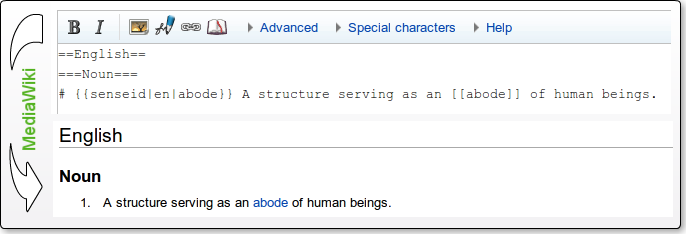
\includegraphics[width=0.9\textwidth]{./images/wikitext.png}
\caption{An excerpt of the \wik page \textit{house} with the rendered HTML.}
\label{fig:wikitext}
\end{figure}

The markup \texttt{==} is used to denote headings, \texttt{\#} denotes a numbered list (\texttt{*} for bullets), \texttt{[[link label]]} denotes links and \texttt{\{\{\}\}} calls a template.
Templates are user-defined rendering functions that provide shortcuts aiming to simplify manual editing and ensuring consistency among similarly structured content elements. 
In MediaWiki, they are defined on special pages in the \texttt{Template:} namespace. 
Templates can contain any wikitext expansion, HTML rendering instructions and placeholders for arguments. 
In the example page in Figure~\ref{fig:wikitext}, the \texttt{senseid} template\footnote{\url{http://en.wiktionary.org/wiki/Template:senseid}} is used, which does nothing being visible on the rendered page, but adds an id attribute to the HTML \texttt{li}-tag (which is created by using \texttt{\#}).
If the English \wik community decides to change the layout of senseid definitions at some point in the future , only a single change to the template definition is required. 
Templates are used heavily throughout \wik, because they substantially increase maintainability and consistency. 
But they also pose a problem to extraction: on the unparsed page only the template name and its arguments are available.
Mostly this is sufficient, but if the template adds static information or conducts complex operations on the arguments (which is fortunately rare), the template result can only be obtained by a running MediaWiki installation hosting the pages. 
The resolution of template calls at extraction time slows the process down notably and adds additional uncertainty.

\subsection{Wiktionary}\label{sec:wiktionary}
\wik has some unique and valuable properties:
\begin{compactitem}
  \item \textbf{Crowd-sourced} \\
    \wik is community edited, instead of expert-built or automatically generated from text corpora. 
    Depending on the activeness of its community, it is up-to-date to recent changes in the language, changing perspectives or new research. 
    The editors are mostly semi-professionals (or guided by one) and enforce a strict editing policy. 
    Vandalism is reverted quickly and bots support editors by fixing simple mistakes and adding automatically generated content. 
    The community is smaller than Wikipedia's but still quite vital (between 50 and 80 very active editors with more than 100 edits per month for the English \wik in 2012\footnote{\url{http://stats.wikimedia.org/wiktionary/EN/TablesWikipediaEN.htm}}). 
   \item \textbf{Multilingual}\\
    The data is split into different Wiktionary Language Editions (WLE, one for each language). 
    This enables the independent administration by communities and leaves the possibility to have different perspectives, focus and localization.
    Simultaneously one WLE describes multiple languages; only the representation language is restricted. 
    For example, the German \wik contains German description of German words \textbf{as well as} German descriptions for English, Spanish or Chinese words. 
    Particularly the linking across languages shapes the unique value of \wik as a rich multi-lingual linguistic resource. 
    Especially the WLE for not widely spread languages are valuable, as corpora might be rare and experts are hard to find.
  \item \textbf{Feature rich}\\
    As stated before, \wik contains for each lexical word (A lexical word is just a string of characters and has no disambiguated meaning yet) a disambiguation regarding language, part of speech, etymology and senses. 
    Numerous additional linguistic properties exist normally for each part of speech. 
    Such properties include word forms, taxonomies (hyponyms, hyperonyms, synonyms, antonyms) and translations.
    Well maintained pages (e.g. frequent words) often have more sophisticated properties such as derived terms, related terms and anagrams.
  \item \textbf{Open license}\\
    All the content is dual-licensed under both the \textit{Creative Commons CC-BY-SA 3.0 Unported License}\footnote{\url{http://en.wiktionary.org/wiki/Wiktionary:Text_of_Creative_Commons_Attribution-ShareAlike_3.0_Unported_License}} as well as the \textit{GNU Free Documentation License (GFDL)}.\footnote{\url{http://en.wiktionary.org/wiki/Wiktionary:GNU_Free_Documentation_License}}
    All the data extracted by our approach falls under the same licences. 
  \item \textbf{Big and growing}\\
    English contains 2,9M pages, French 2,1M, Chinese 1,2M, German 0,2 M.
    The overall size (12M pages) of \wik is in the same order of magnitude as Wiki\-pedia's size (20M pages)\footnote{\url{http://meta.wikimedia.org/wiki/Template:Wikimedia_Growth}}. 
    The number of edits per month in the English \wik varies between 100k and 1M --- with an average of 200k for 2012 so far. 
    The number of pages grows --- in the English \wik with approx. 1k per day in 2012.\footnote{\url{http://stats.wikimedia.org/wiktionary/EN/TablesWikipediaEN.htm}}
\end{compactitem}
\vspace{0.5cm}
The most important resource to understand how \wik is organized are the \textit{Entry Layout Explained} (ELE) help pages.
As described above, a page is divided into sections that separate languages, part of speech etc. 
The table of content on the top of each page also gives an overview of the hierarchical structure. 
This hierarchy is already very valuable as it can be used to disambiguate a lexical word. 
The schema for this tree is restricted by the ELE guidelines\footnote{For English see \url{http://en.wiktionary.org/wiki/Wiktionary:ELE}}. 
The entities illustrated in Figure~\ref{fig:example} of the ER diagram will be called \textit{block} from now on. 
The schema can differ between WLEs and normally evolves over time.

\begin{figure}[htb]
\centering
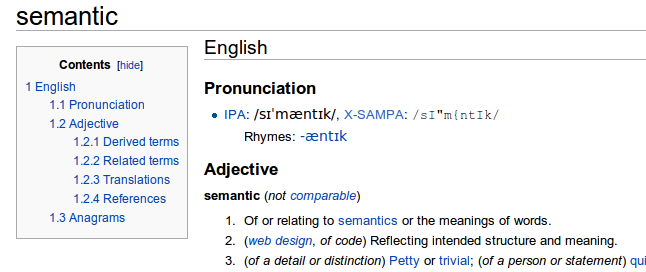
\includegraphics[width=0.9\textwidth]{./images/example-page.png}
\vspace{0.3cm}
\hspace{0.1cm}
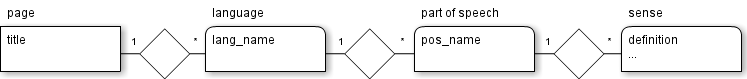
\includegraphics[width=0.9\textwidth]{./images/entrylayout.png}
\caption{Example page \texttt{http://en.wiktionary.org/wiki/semantic} and underlying schema (only valid for the English \wik, other WLE might look very different.)}
\label{fig:example}
\end{figure}

\subsection{Wiki-scale Data Extraction}
The above listed properties that make \wik so valuable, unfortunately pose a serious challenge to extraction and data integration efforts. 
Conducting an extraction for specific languages at a fixed point in time is indeed easy, but it eliminates some of the main features of the source. 
To fully synchronize a knowledge base with a community-driven source, one needs to make distinct design choices to fully capture all desired benefits.
MediaWiki was designed to appeal to non-technical editors and abstains from intensive error checking as well as formally following a grammar --- the community gives itself just layout guidelines. 
One will encounter fuzzy modelling and unexpected information. 
Editors often see no problem with such "noise" as long as the page's visual rendering is acceptable.  
Overall, the issues to face can be summed up as 
\begin{enumerate}
\item the constant and frequent changes to data \textit{and schema},
\item the heterogeneity in WLE schemas and
\item the human-centric nature of a wiki.
\end{enumerate}  
From perspective of requirements engineering, they result in a number of requirements, that do not easily fit together. Figure \ref{fig:requirements} illustrates the different requirements.
\begin{figure}[tb]
\centering
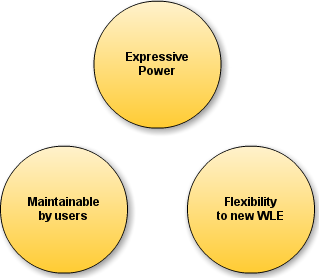
\includegraphics[width=0.4\textwidth]{../images/requirements}
\caption{Competing requirements in wiki scale data extraction}
\label{fig:requirements}
\end{figure}
The requirement "Expressiveness" is the sum of all functional requirements. The other two are non-functional as they regard the long term sustainability of the development process.
Approaches with hard coded algorithms mostly cover only the first requirement. If a modular architecture is used, it might be easy to cover the "Flexibility to new WLE"; a extractor for each WLE might be hard coded. Although it might be arguable whether the growing code base stays maintainable, with sufficient effort of software developers, such an approach theoretically could scale. However development costs could be reduced drastically if the extraction is maintained by users. The two non-functional requirements conflict with expressiveness as they are implemented with a declarative pattern in our case (and I argue that it is essential to do so, because only a declarative approach can hide the complexity). The more feature the declarative language supports, the harder it becomes for non experts to use it. In section \ref{sec:implementation} it will be shown which trade off is chosen. 


\newpage


\section{Specification}
\label{sec:specification}
\subsection{Overview}
In the following I will describe the used architecture. 

Existing extractors as presented in Section~\ref{relatedWork} mostly suffer from their \textit{inflexible} nature resulting from their narrow use cases at development time. 
Very often approaches were only implemented to accomplish a short term goal (e.g. prove a scientific claim) and only the needed data was extracted in an \emph{ad-hoc} manner. 
Such evolutionary development generally makes it difficult to generalize the implementation to heterogeneous schemas of different WLE.
Most importantly, however, they ignore the community nature of a \wik. 
Fast changes of the data require ongoing maintenance, ideally by the wiki editors from the community itself or at least in tight collaboration with them.
These circumstances pose serious requirements to software design choices and should not be neglected. 
All existing tools are rather monolithic, hard-coded black boxes. 
Implementing a new WLE or making a major change in the WLE's ELE guidelines will require a programmer to refactor most of its application logic. 
Even small changes like new properties or naming conventions will require software engineers to align settings. 
The amount of maintenance work necessary for the extraction correlates with change frequency in the source. 
Following this argumentation, a community-built resource can only be efficiently extracted by a community-configured extractor. 
This argument is supported by the successful crowd-sourcing of DBpedia's internationalization~\cite{Kontokostas2012}  and the non-existence of \textit{open} alternatives with equal extensiveness.\\
Given these findings, we can now conclude four high-level design goals:
\begin{compactitem}
\item declarative description of the page schema;
\item declarative information/token extraction, using a terse syntax, maintainable by non-programmers;
\item configurable mapping from language-specific tokens to a global vocabulary;
\item fault tolerance (uninterpretable data is skipped).
\end{compactitem}

The extractor is built on top of the the DBpedia framework, and thus it is required to conform to a simple interface:

\begin{figure}[tb]
\centering
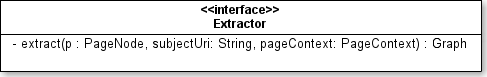
\includegraphics[width=0.6\textwidth]{./images/interface.png}
\caption{The extractor interface.}
\label{fig:interface}
\end{figure}

Extractors are registered with the framework via a configuration file, and instantiated with a requested context. The context can be the DBpedia ontology or the selected language etc. Extractors are then subsequently invoked for every page of the MediaWiki XML dump. They are given the page in parsed form of an AST, subjectURI the URI of the resource this page should be referring to (\texttt{http://dbpedia.org/resource/\$PAGENAME}) and pageContext --- a helper for URI generation. The interface defines the extractor to return a Graph in turn, which is basically a set of triples (or quads in this case). Internally the extractor will inspect the AST and generate triples, when he finds information he interprets as relevant. This straightforward interface makes the DBpedia framework so modular. Input and output handling (parsing and serialization) is left to the framework, and the resulting RDF data can be directly inserting into an triple store.

We solve the above requirements with an additional extractor, which internally follows a rather sophisticated workflow, shown in Figure~\ref{fig:architecture}.

\begin{figure}[tb]
\centering
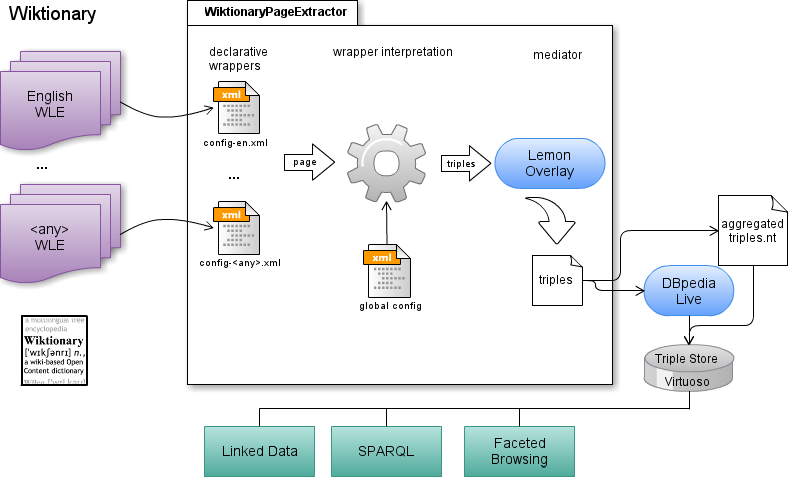
\includegraphics[width=0.9\textwidth]{./images/architecture.png}
\caption{Architecture for extracting semantics from Wiktionary leveraging the DBpedia framework.}
\label{fig:architecture}
\end{figure}
The \wik extractor is invoked by the DBpedia framework to handle a page.
It uses a language-specific configuration file, that has to be tailored to match the WLE's ELE guidelines to interpret the page, to extract the desired information. 
At first, the resulting triples still adhere to a language-specific schema, that directly reflects the configured layout of the WLE. 
A generic lossless transformation and annotation using the \lemon vocabulary is then applied to enforce a global schema and reduce semantic heterogeneity. 
Afterwards the triples are returned to the DBpedia frameworks, which takes care of the serialization and (optionally) the synchronization with a triple store via DBpedia Live\footnote{\url{http://live.dbpedia.org/live}}.
%TODO optional cite live
The process of interpreting the declarative wrapper is explained in more detailed in Figure~\ref{fig:extractor}.

\begin{figure}[tb]
\centering
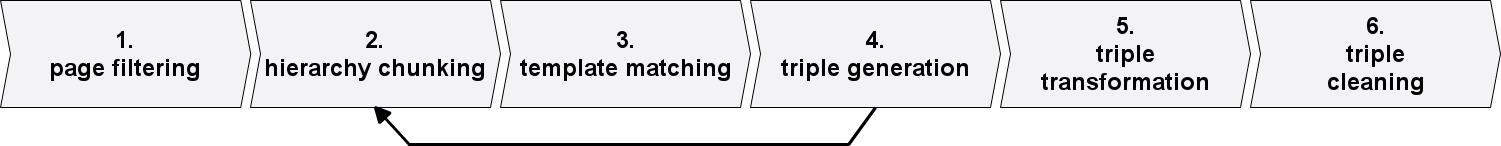
\includegraphics[width=0.9\textwidth]{./images/extractor.png}
\caption{Overview of the extractor workflow.}
\label{fig:extractor}
\end{figure}



\vfill
\newpage


\section{Design and Implementation}
\label{sec:implementation}
In the following I will present a bunch of noteworthy implementation details.

\subsection{Extraction Templates}\label{sec:extpl}
As mentioned in Section~\ref{sec:wiktionary}, we define \textit{block} as the part of the hierarchical page that is responsible for a certain entity in the extracted RDF graph. 
For each \textit{block}, there can be declarations on how to process the page on that level.
This is done by so called \textit{extraction templates} (called \textit{ET}; not to be confused with the templates of \textit{wikitext}).
Each possible section in the \wik page layout (i.e. each linguistic property) has an ET configured (explained in detail below). 
The idea is to provide a declarative and intuitive way to encode \textit{what to extract}.
For example consider the following page snippet:
\begin{lstlisting}
===Synonyms===
* [[building]]
* [[company]]
\end{lstlisting}
Since the goal is to emit a triple for each link per line, we can write the ET in the following style:
\begin{lstlisting}
===Synonyms===
(* [[\$target]]
)+
\end{lstlisting}
Lets analyse what features are available to build ET:\newline
\textbf{Template matching:}
To match a template against a page, both are compared node by node:
\begin{figure}[h]
\centering
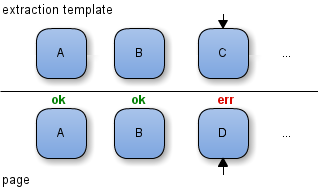
\includegraphics[width=0.4\textwidth]{../images/matching}
\caption{Matching a extraction template against a page}
\label{fig:matching}
\end{figure}
Internally a \texttt{Stack}\footnoteUrl{http://www.scala-lang.org/api/current/scala/collection/mutable/Stack.html} is used; if the head nodes of both stacks are equal, they are consumed, if not an \texttt{Exception} is thrown to notify about a mismatch.\newline
\textbf{Variables:}
In the extraction template, there can be special nodes (e.g. variables). 
If a variable is encountered, all nodes from the page are being recorded and saved as a binding for that variable. 
All bindings that are saved within a extraction template are collected and returned as a result of the template being matched against the page.
\begin{figure}[h]
\centering
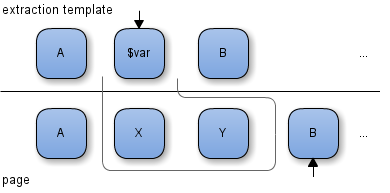
\includegraphics[width=0.4\textwidth]{../images/varbinding}
\caption{recording a variable}
\label{fig:varbinding}
\end{figure}
Some short notes about variables:
\begin{compactitem}
\item the pattern to recognize them is \texttt{\textbackslash\$[a-zA-Z0-9]}
\item they stop recording the page when they encounter the token, that follows the variable in the extraction template
\item if there is no node following them, they consume everything
\item if they record too many nodes (the whole page), they are assumed to be faulty and an exception is thrown
\end{compactitem}
\textbf{Repetition:}
The possibility to have a subtemplate that can be repeated. 
Delimited by \texttt{(} \ldots \texttt{)} and succeeded with one of three modifiers:
\begin{compactitem}
\item \texttt{*} for \textit{0..n} matches,
\item \texttt{+} for \textit{1..n} matches and 
\item \texttt{?} for \textit{0..1} matches.
\end{compactitem}
How do variables relate to repetitions? If a variable is used in a repetition and bound twice, it doubles the number of varbindings. 
Variables outside the repetition are then duplicated. Formalized: the flattened version of the (directed) \textit{binding tree} is the \textit{set of all paths} starting at the root.
\begin{figure}[htbp]
\centering
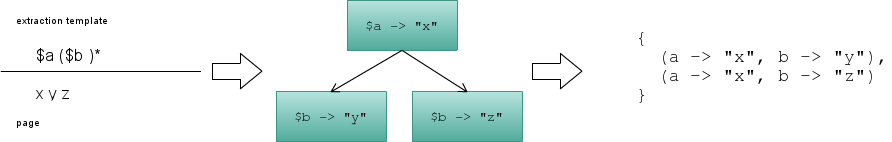
\includegraphics[width=0.8\textwidth]{../images/varlist}
\caption{using variables in repetitions}
\label{fig:varlist}
\end{figure}\newline
\textbf{Error tolerance:}
Due to the human-centric nature of a wiki, pages often contain unexpected information: an additional image, a editor note or a rare template. 
To compensate this, we decided to add the possibility to weaken the conditions for a template mismatch. 
When a node is encountered on the page, that is not expected from the template, the template it is not immediately aborted, but instead it is noted that there was a error and this unexpected node is skipped. 
To limit these skips, a window over the last \textit{s} nodes is observed, to calculate a error threshold \textit{maxError}. 
This allows the template to recover from local errors if it later continues to match. 
Additionally the edge case of templates with length 0 or 1 and 1 unexpected node, should be avoided to succeed by the \textit{minCorrect} parameter that prevents templates from matching too easily.
\begin{figure}[h]
\centering
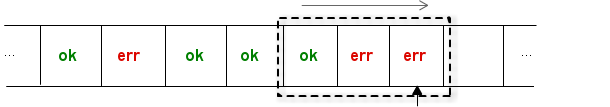
\includegraphics[width=0.8\textwidth]{../images/sliding}
\caption{Error tolerance with a sliding window ($\textit{s}=3, \textit{minCorrect}=1, \textit{maxError}=1)$}
\label{fig:sliding}
\end{figure}
The example shows how confined errors (the single one) are ignored but major errors (like the two consecutive ones) will prevent the template from matching.
This implements a sliding window as only the last \textit{s} nodes are considered and this window progresses with the page being consumed.\newline
These are the most important features of extraction templates.\newline
Back to our example:
The found \textit{variable bindings} are \texttt{\{(\$target -> "building"), (\$target -> "company")\}}. 
How do we transform these bindings into RDF triples? We simply invert the idea of extraction templates to \textit{result templates} (called RT). We insert the value of variables into subject, predicate and object of a RDF triple:
\begin{lstlisting}[style=XML]
<triple s="http://some.ns/$entityId" p="http://some.ns/hasSynonym" o="http://some.ns/$target" />
\end{lstlisting}
Notice the reuse of the \texttt{\$target} variable:
The data extracted from the page is inserted into a triple.
The variable \texttt{\$entityId} is a reserved global variable, that holds the page name i.e. the word.
The created triples in N-Triples syntax are:
\begin{lstlisting}[style=N3]
<http://some.ns/house-1>   <http://some.ns/hasSynonym>   <http://some.ns/building> .
<http://some.ns/house-1>   <http://some.ns/hasSynonym>   <http://some.ns/company> .
\end{lstlisting}
The used RT can be more complex (as explained below).

\subsection{Algorithm}
The algorithm of processing a page works as follows:

\textit{Input:} Parsed page obtained from the DBpedia Framework (essentially a lexer is used to split the Wiki Syntax into tokens)
\begin{enumerate}
\item Filter irrelevant pages (user/admin pages, statistics, list of things, files, templates, etc.) by applying string comparisons on the page title. 
Return an empty set of triples in that case.
\item Build a finite state automaton\footnote{Actually a finite state transducer, most similar to the Mealy-Model.} from the page layout encoded in the WLE specific XML configuration. 
This schema also contains so called \textit{indicator templates} for each \textit{block}, that --- if they match at the current page token --- indicate that their respective block starts. 
So they trigger state transitions. 
In this respect the mechanism is similar to \cite{McCrae_2012}, but in contrast our approach is declarative --- the automaton is constructed \textit{on-the-fly} and not hard-coded. 
The current state represents the current position in the disambiguation tree.
\item The page is processed token by token:
\begin{enumerate}
\item Check if \textit{indicator templates} match. 
If yes, the corresponding block is entered. 
The \textit{indicator templates} also emit triples like in the \textit{extraction template} step below. 
These triples represent the block in RDF -- for example the resource \url{http://wiktionary.dbpedia.org/resource/semantic-English} represents the English block of the page "semantic".
\item Check if any \textit{extraction template} of the current block match.
\subitem If yes, transform the variable bindings to triples.\footnote{In our implementation: 
Either declarative rules are given in the XML config or alternatively static methods are invoked on user-defined classes (implementing a special interface) for an imperative transformation. This can greatly simplify the writing of complex transformation.} Localization specific tokens are replaced as configured in the so called \textit{language mapping} (explained in detail in section \ref{sec:mapping}).
\end{enumerate}
\item The triples are then \textit{transformed}. 
In our implementation \textit{transformation} means, that all triples are handed to a static function, which return a set of triples again. 
One could easily load the triples into a triple store like JENA and apply arbitrary SPARQL Construct and Update transformations. 
This step basically allows post-processing, e.g. consolidation, enrichment or annotation. 
In our case, we apply the schema transformation (by the mediator) explained in detail in Section \ref{sec:lemon}).
\item The triples are sorted and de-duplicated to remove redundancy in the RDF dumps.
\end{enumerate}
\textit{Output:} Set of triples (handed back to the DBpedia Framework).

\subsection{Language Mapping}\label{sec:mapping}
The language mappings are a very simple way to translate and normalize tokens, that appear in a WLE. 
In the German WLE, for example, a noun is described with the German word "\textit{Substantiv}". 
Those tokens are translated to a shared vocabulary, before emitting them (as URIs for example). 
The configuration is also done within the language specific XML configuration:
\begin{lstlisting}[style=XML]
 <mapping from="Substantiv" to="Noun"> 
 <mapping from="Deutsch" to="German"> 
 ...
\end{lstlisting}
The mapping consists currently of mappings for part of speech types and languages. 
But arbitrary usage is possible. 
Section~\ref{sec:functions} shows how this mapping is used.

\subsection{Reference Matching}\label{sec:matching}
A \wik specific requirement is the resolution of intra-page references: All Wiktionaries use \textit{some} way to refer to parts of the traits of the word. 
For example on the page \textit{house} at first senses are defined:
\begin{lstlisting}[basicstyle=\tiny\ttfamily]
# A structure serving as an [[abode]] of human beings.
# {{politics}} A deliberative assembly forming a component of a legislature, or, more rarely, the room or building in which such an assembly normally meets.
# [[house music|House music]].
\end{lstlisting}
Later on relations to other words are noted --- but \textit{in context} of a sense. 
For example house \textit{in context} of \textit{abode} has the translation \textit{Haus} in German. So the following notion is used:
\begin{lstlisting}[basicstyle=\tiny\ttfamily]
====Translations====
{{trans-top|abode}}
...
* German: {{t+|de|Haus|n}}, {{t+|de|Häuser|p}}
...
\end{lstlisting}
The problem is to match the gloss that is given in the \texttt{trans-top} template argument against the available senses.
The senses have been asigned URIs already; now those are needed to serve as subject for the translation triples. There is no simple way to determine which sense URI belongs to which gloss. 
As described in \cite{meyer_2011b} as \textit{relation anchoring}, a string based measure is used\footnote{Opposed to the approach described in \cite{meyer_2011b}, we try to focus on explicit information. Determining the sense URI of a translation triple is already error prone, but so called \textit{target anchoring} is not performed. 
\textit{Target anchoring} refers to the disambiguation of the target word (or entity): this target of course has also a disambiguation tree, and it is possible to \textit{bend} the link to point to a node deeper in that tree instead of just the root node. 
We consider this highly assumptious and it introduces noise. 
We leave that to postprocessing. 
Also it is not implementable easily within the DBpedia framework, because data extracted on other pages is not available to a extractor at runtime.}. 
There is a simple data structure that is initialized per page, to this matching mechanism. Which measure is used can be configured in the global configuration. 
Available measures are: Levenshtein and trigram set similarity with dice, jaccard or overlap coefficient. 
A sense can be registered with the matcher by passing its definition sentence. 
An \textit{id} is generated for that sense. 
Later on, glosses (short forms of the definition) that refer to a sense can be passed to lookup which sense matches best, and the corresponding \textit{id} is returned. 
Opposed to existing approaches we make no assumptions on how such references are noted. 
The English \wik uses glosses, the German one uses explicit numbers (that don't need to be matched), the Russian and French uses a combination of both --- sometimes senses are explicitly referred to by their numbers, sometimes with a gloss. 
So we came up with a customizable way to use the reference matcher. 
Section~\ref{sec:functions} shows how this mechanism is used.

\subsection{Formatting functions in Result Templates}\label{sec:functions}
The question arises, how this mapping is then used within the application. 
It is certainly not reasonable to replace \textit{all} occurrences of those \texttt{from} tokens. This would lead to a number of false positive matches and screwed output. 
It is crucial to offer a possibility to configure in which context output should be handled so.
I therefore introduced formatting functions in result templates: when you note the triples that are generated you can apply functions to e.g. variables. 
An example:
\begin{lstlisting}[style=XML]
<triple s="http://some.ns/uri($entityId)" p="http://some.ns/hasLanguage" o="http://some.ns/map($target)" />
\end{lstlisting}
In this RT, two functions are used: \texttt{uri} and \texttt{map}. 
They are wrapped around variable parts, and on rendering they are resolved. 
The following functions are available:\\
\begin{table}[h!] 
\centering 
\begin{tabular}{|l|l|}
\hline \texttt{uri(str)} & URL encode \\ 
\hline \texttt{map(str)} & replace if mapping found \\ 
\hline \texttt{assertMapped(str)} & dont emit triple if not in mapping vocabulary \\ 
\hline \texttt{assertNumeric(str)} & dont emit triple if argument is not numeric \\ 
\hline \texttt{getId(str)} & lookup a gloss and return the id of the best matching sense \\ 
\hline \texttt{getOrMakeId(str)} & lookup a id or generate one if below a similarity threshold \\ 
\hline \texttt{makeId(str)} & save a sense and generate an id \\ 
\hline \texttt{saveId(str, str)} & save a sense with a given id \\ 
\hline 
\end{tabular} 
\end{table}
The functions with \textit{Id} in their name relate to the matching introduced in section~\ref{sec:matching}. 
Continuing the example of senses and translations, one would write the RT in a way to save definition sentences when generating them as triples and later matching the gloss, when generating triples about the translation section:
For the defintions
\begin{lstlisting}[style=XML]
<triple s="http://some.ns/$entityId-makeId($definition)" p="http://some.ns/hasDefinition" o="$definition" oType="literal" />
\end{lstlisting}
and for the translations
\begin{lstlisting}[style=XML]
<triple s="http://some.ns/$entityId-getId($gloss)" p="http://some.ns/hasTranslation" o="http://some.ns/uri($target)" />
\end{lstlisting}
The idea is that (if the matching is correct), the subject URIs are equal (e.g. \url{http://some.ns/house-1}) in both triples --- there are two triples about one resource --- information successfully merged.
\begin{lstlisting}[style=N3]
<http://some.ns/house-1>   <http://some.ns/hasDefinition>   "A structure serving as an abode of human beings." .
<http://some.ns/house-1>   <http://some.ns/hasTranslation>   <http://some.ns/Haus> .
\end{lstlisting}
 
\subsection{Schema Mediation by Annotation with \lemonnospace}
\label{sec:lemon}
The last step of the data integration process is the schema normalization.
The global schema of all WLE is not constructed in a centralized fashion --- instead we found a way to both making the data globally navigable and keeping the heterogeneous schema without loosing information.
\lemonnospace~\cite{lemon-eswc} is an RDF model for representing lexical information (with links to ontologies --- possibly DBpedia). 
We use part of that model to encode the relation between \textit{lexical entries} and \textit{lexical senses}.
\lemon has great potential of becoming the \textit{de facto} standard for representing dictionaries and lexica in RDF and is currently the topic of the OntoLex W3C Community group\footnote{\url{http://www.w3.org/community/ontolex/}}. 
The rationale is to add \textit{shortcuts} from \textit{lexical entities} to \textit{senses} and propagate properties that are along the intermediate nodes down to the senses.
This can be accomplished with a generic algorithm (a generic tree transformation, regardless of the depth of the tree and used links).
Applications assuming only a \textit{lemon} model, can operate on the shortcuts and (if applied as an overlay --- leaving the original tree intact) this still allows applications, to also operate on the actual tree layout.
The (simplified) procedure is presented in Figure~\ref{fig:lemon}\footnote{Note, that in the illustration it could seem like the information about part-of-speech would be missing in the \textit{lemon} model. This in not the case. Actually from the part-of-speech nodes, there is a link to corresponding language nodes.
These links are also propagated down the tree.}. 
\begin{figure}[tb]
\centering
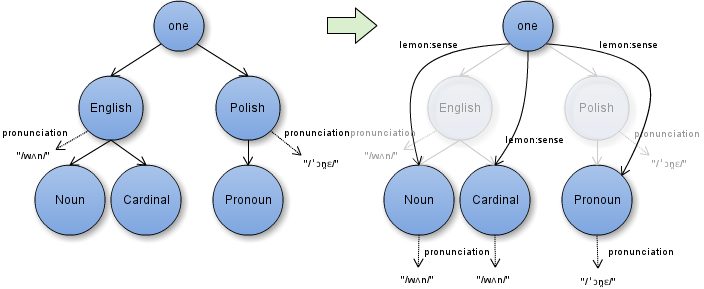
\includegraphics[width=\textwidth]{./images/lemon.png}
\caption{Schema normalization.}
\label{fig:lemon}
\end{figure}
The use of the \lemon vocabulary and model as an additional schema layer can be seen as our mediator.
This approach is both lightweight and effective as it takes advantage of \textit{multi-schema modelling}.

\subsection{Configuration}
As presented in section \ref{sec:requirements}, the most important requirement of the approach is configurability. The extractor itself is as generic as possible, it is not tailored to linguistics or even \wik. 
It has commitment to wiki syntax, but is also able to process plain text as it can be interpreted as wikitext without markup, thus the extractor may be suitable for most flat file formats. 
However the configuration makes up the heart of the extractor: it is a big XML file interpreted at runtime and describes how to interpret the page. 
I will go through the available options and show their relevance to the given requirements.

At first the configuration is splitted into a generic part and a language specific part. 
The generic part is always loaded and does not need to be localized to a WLE. 
It contains options like the namespace, in which all URIs are created and an option that specifies which language configuration should be used. 
The language specific configuration is loaded based on that option at runtime. 
It has to be tailored to a WLE by the maintainer of the dataset.

Both configuration types are stored in the \texttt{config} folder. 
The naming convention restricts the folder to like the following:
\dirtree{%
.1 config.
.2 config.xml.
.2 config-de.xml.
.2 config-en.xml.
.2 \ldots.
}

The generic configuration has two parts: a properties list and a mapping. 
The properties are the mentioned namespace, the language, the \texttt{loglevel} (to configure debug verbosity) and options to configure the matcher. 
The mapping is --- as explained in section~\ref{sec:mapping} --- a way to replace tokens found on the page to a global vocabulary. 
But opposed to language specific tokens, in the generic configuration, globally used tokens are configured. 
It is used to provide a mapping from ISO 639-1 and -2 codes to the \wik vocabulary.

\begin{lstlisting}[style=XML]
<?xml version="1.0" encoding="UTF-8"?>
<config>
    <properties>
        <property name="logLevel" value="0"/>
        <property name="language" value="ru"/>
        <property name="ns" value="http://wiktionary.dbpedia.org/"/>
        <property name="matchingStrategy" value="levenshtein"/>
        <property name="matchingThreshold" value="0.5"/>
    </properties>
    <mappings>
        <!-- ISO 639-1 -->
        <mapping from="aa" to="Afar" />
        <mapping from="ab" to="Abkhazian" />
        <mapping from="ae" to="Avestan" />
        ...
\end{lstlisting}

The language specific configuration is probably the most important part of this thesis. 
The created XML dialect directly reflects the expressiveness of the extraction approach. 
As explained in section \ref{sec:requirements}, the expressiveness is limited by the complexity of the declarative language. 
However he declarative language should remain simple to keep it easily usable by non experts. 
The interpreter should be as generic as possible. 
In the following I will present which trade off was chosen and how the layout of a WLE is modelled in our XML dialect.

The configuration for English should serve as an example here\footnoteUrl{http://dbpedia.hg.sourceforge.net/hgweb/dbpedia/extraction_framework/file/c871ba718cf6/wiktionary/config/config-en.xml}. 
The XML is structured as
\dirtree{%
.1 <config>.
.2 <ignore>.
.2 <mappings>.
.2 <postprocessing>.
.2 <saveVars>.
.2 <templateRepresentativeProperties>.
.2 <page>.
}

The \texttt{<ignore>} section configures which pages shall be skipped and not used for extraction. 
This is used to skip help pages or user profiles, but it can be also used to skip pages like conjugation tables, as they are not handled yet. 
An example for this section could be
\begin{lstlisting}[style=XML]
<ignore>
	<page startsWith="Help:" />
	<page endsWith=" (Conjugation)" />
	...
\end{lstlisting}
There are two options to determine if a page should be skipped: Prefix or suffix matches in the page title.

The mappings section has been explained in \ref{sec:mapping}, it is used to translate language specific terms for languages or part of speech types and can be invoked by formatting functions in result templates as explained in \ref{sec:functions}.\newline
\texttt{<postprocessing>} configures whether and how the extracted triples of a page should be handled. 
It is possible to pass them to so called \texttt{Postprocessors} (that are JVM classes, visible in classpath, that need to implement a certain interface \texttt{Postprocessor}). 
This \texttt{Postprocessor} can be configued by arbitrary XML nodes. 
The interpretion of those is left to the class itself. 
An example for \texttt{Postprocessors} is the lemon overlay. 
It is invoked like this:
\begin{lstlisting}[style=XML]
<postprocessing enabled="true" ppClass="org.dbpedia.extraction.mappings.wikitemplate.wiktionary.postprocessor.LemonOverlay">
  <config>
    <blockProperty uri="http://www.monnet-project.eu/lemon#sense"/>
    <inputTargetClass uri="http://wiktionary.dbpedia.org/terms/Sense"/>
    <followProperties>
      <property uri="http://wiktionary.dbpedia.org/terms/hasPoSUsage"/>
      <property uri="http://wiktionary.dbpedia.org/terms/hasLangUsage"/>
      <property uri="http://wiktionary.dbpedia.org/terms/hasSense"/>
    </followProperties>
    <collectProperties>
      <property uri="http://purl.org/dc/elements/1.1/language"/>
      <property uri="http://www.w3.org/2000/01/rdf-schema#label"/>
      <property uri="http://wiktionary.dbpedia.org/terms/hasMeaning"/>
      <property uri="http://wiktionary.dbpedia.org/terms/hasTranslation"/>
      <property uri="http://wiktionary.dbpedia.org/terms/hasExampleSentence"/>
      ...
    </collectProperties>
    <outputStartClass uri="http://www.monnet-project.eu/lemon#LexicalEntry"/>
    <outputAggregatedClass uri="http://www.monnet-project.eu/lemon#LexicalSense"/>
  </config>
</postprocessing>
\end{lstlisting}

\texttt{<saveVars>} allows to cache variables between template matches. 
Normally the only variables visible in result templates, are the ones bound in the extraction templates. 
We extended this with a cache, so certain variables can be kept. 
If a variable is set to be saved like this
\begin{lstlisting}[style=XML]
<saveVars>
  <var name="pos"/>
  <var name="language"/>
  <var name="definition"/>
</saveVars>
\end{lstlisting}
its last value stays available to be used in further result templates. In other words: after being bound, the variable stays visible --- gets a global scope. 
This memory allows for a kind of context sensitivity by means of \textit{look back}. 
The mechanism is currently not used.\newline
\texttt{templateRepresentativeProperties} works as a very simple \textit{template resolution} mechanism. 
To resolve templates (render them to readable text), actually a running MediaWiki instance is necessary. 
But often this is superfluous: it might be sufficient to simply choose a argument of that template to represent it readable. 
For example the English template \texttt{term} is used to format links to other words; it is printed as the word itself which is the first argument. 
Other information can be ignored. 
So I came up with this simple but effective mechanism to note which property is used to represent templates:
\begin{lstlisting}[style=XML]
<templateRepresentativeProperties>
  <templateRepresentativeProperty tplName="term" pKey="1"/>
  ...
  <templateRepresentativeProperty tplName="proto" pKey="2"/>
</templateRepresentativeProperties>
\end{lstlisting}

Finally we come to the most important section: the \texttt{page} section. 
It describes the overall layout of a page within a WLE.
As defined in section~\ref{sec:wiktionary}, a page is hierarchically divided into \textit{blocks}. 
The need arises to configure
\begin{enumerate}
\item the hierarchy of the blocks
\item how the start of a block is recognized
\item which extraction templates are used in each block
\end{enumerate}

The first is achieved by nesting \texttt{<block>} nodes into each other:
\begin{lstlisting}[style=XML]
<page>
  <block name="language">
    <block name="pos>
      ...
    </block>
  </block>
</page>
\end{lstlisting}

The second is realised by reusing templates. 
As introduced above, templates are matched against the page; additionally to extracting triples, they are here used to react \textit{when} they match. 
A block can have several templates configured and while the extractor scans the page, it tries to match these \textit{indicator templates}.
If they match, they trigger the start of a block. In the next step we will see how such a template is actually configured. 
The syntax for extraction templates and indicator templates is exactly the same\footnote{the interpreting code is reused}. 
The indicator templates are stored in each block:
\begin{lstlisting}[style=XML]
<block name="language">
  <indicators>
    <indicator>
      ... (see below)
    </indicator>
  </indicators>
  ...
</page>
\end{lstlisting}

The third is done by the \texttt{templates} section within each block:
\begin{lstlisting}[style=XML]
<block name="language">
  <indicators />
  <templates>
    <template name="example">
      <wikiTemplate>===Etymology=== 
$etymology
</wikiTemplate>
      <resultTemplates>
        <resultTemplate>
          <triples>
            <triple s="$block" p="http://wiktionary.dbpedia.org/terms/hasEtymology" o="$etymology" oType="literal"/>
          </triples>
        </resultTemplate>
      </resultTemplates>
      </template>
    </template>
  </templates>
</page>
\end{lstlisting}
The basics were explained in section~\ref{sec:extpl}, now we put them together: the \texttt{<template>} node is divided into two parts --- the extraction template in \texttt{<wikiTemplate>} and the result templates.

The \textit{extraction template} has been explained already above. 
It is put in the \texttt{<wikiTemplate>} node --- only thing to keep in mind there is whitespace: whitespaces count, also every indention or linebreak will be interpreted as wiki text. 
Make sure you don't accidentally change the template, because it will most likely not match anymore.
Also set your text editor to show control characters like spaces, tabs, or newlines (cf. the $\P$ symbol).

Additionally to the \textit{result template} basics introduced above, for a \texttt{<template>} there can be multiple RT and each consist of a set of triple templates. 
The rational is to respect missing bindings: if a variable is inside a optional repetition, it may not be present in the variable bindings. 
If those bindings are then converted to triples by a \textit{result template}, missing variables will result in the current triple to fail. 
To avoid inconsistent triples (because some are missing), then all triples shall not be emitted. 
Thus result templates are atomic --- either all triples inside are emitted or none. 
This allows to model triples separately for varying page content \textit{within one template}.
Another way to respect diverse layouts, is to declare a triple \textit{optional}:
\begin{lstlisting}[style=XML]
<resultTemplate>
  <triple s="http://some.ns/$entityId" p="http://some.ns/hasSense" o="http://some.ns/$entityId-$sense" />
  <triple s="http://some.ns/$entityId-$sense" p="http://some.ns/hasSource" o="$source" optional="true" />
</resultTemplate>
\end{lstlisting}
This disregards a missing variable --- the result template will still succeed if the optional triple fails.

A very important feature is the global \texttt{\$block} variable together with the \texttt{oNewBlock} configuration option within \textit{indicator templates}:
Global variables have already been introduced by the \texttt{\$entityId} variable and the possibility to save variables between templates. 
The \texttt{\$entityId} variable is static, it keeps it value over time. 
Saved variables are local variables that become global. 
Now we introduce the \texttt{\$block} variable, that holds the URI of the current block. 
For example if the extractor currently processes the language block of a word the value could be \url{http://some.ns/Haus-German}. 
This value can then be used to construct URIs that reuse this as a prefix:
\begin{lstlisting}[style=XML]
<triple s="$block" p="http://some.ns/hasPosUsage" o="$block-$pos" oNewBlock="true" />
\end{lstlisting}
The object URI could be \url{http://some.ns/Haus-German-Noun} for example. 
But furthermore, if this RT is used within an \textit{indicator template}, the need arises to indicate the start of a new block. 
When I introduced \textit{indicator templates} above --- i lied: not the successful match of template triggers the state change, but only the successfull rendering of a triple with \texttt{oNewBlock} option. 
The rational is, that to trigger that transition, the new URI has to be known --- and there is no simple way to determine it from a set of unremarkable triples that are produced by the indicator template.
Of couse the \texttt{\$block} variable can be used independently from the \texttt{oNewBlock} option in ordinary RT.
\newpage



\section{Evaluation}
\label{sec:evaluation}
The extraction has been conducted as a proof-of-concept on four major WLE:
The English, French, Russian and German \wik.
The datasets combined contain more than 100 million facts\footnote{SPARQL: \texttt{SELECT COUNT(*) WHERE {?s ?p ?o}}} about 5 million lexical words\footnote{SPARQL: \texttt{SELECT COUNT(?s) WHERE {?s a lemon:LexicalEntry}}} .
The data is available as N-Triples dumps\footnote{\url{http://downloads.dbpedia.org/wiktionary}}, Linked Data\footnote{for example \url{http://wiktionary.dbpedia.org/resource/dog}}, via the \emph{Virtuoso Faceted Browser}\footnote{\url{http://wiktionary.dbpedia.org/fct}} or a SPARQL endpoint\footnote{\url{http://wiktionary.dbpedia.org/sparql}}.
The has extraction been conducted on August 15th 2012, and the used XML dumps were the latest as of that day\footnote{In detail: en - 08/12, fr - 08/12, ru - 08/06, de - 08/11}.

\subsection{Example Data}
Just for reference, I present some sample data. It is extracted from the English Wiktionary entry for \textit{goggles}\footnoteUrl{http://en.wiktionary.org/wiki/googles}:
\begin{lstlisting}[style=N3]
@prefix rdf: <http://www.w3.org/1999/02/22-rdf-syntax-ns#>.
@prefix rdfs: <http://www.w3.org/2000/01/rdf-schema#>.
@prefix wt: <http://wiktionary.dbpedia.org/terms/>.
@prefix wr: <http://wiktionary.dbpedia.org/resource/>.
@prefix dc: <http://purl.org/dc/elements/1.1/>.
@prefix doap: <http://usefulinc.com/ns/doap#>.
@prefix lemon: <http://www.monnet-project.eu/lemon#>

wr:goggles doap:creator <http://en.wiktionary.org/w/index.php?title=goggles&action=history> . 
wr:goggles lemon:sense wr:goggles-English-Noun-1en . 
wr:goggles rdfs:label "goggles"@en . 
wr:goggles rdfs:seeAlso <http://ko.wiktionary.org/wiki/goggles> . 
wr:goggles rdfs:seeAlso <http://fi.wiktionary.org/wiki/goggles> . 
wr:goggles rdfs:seeAlso <http://sv.wiktionary.org/wiki/goggles> . 
wr:goggles rdfs:seeAlso <http://io.wiktionary.org/wiki/goggles> . 
wr:goggles rdfs:seeAlso <http://te.wiktionary.org/wiki/goggles> . 
wr:goggles rdfs:seeAlso <http://zh.wiktionary.org/wiki/goggles> . 
wr:goggles rdfs:seeAlso <http://de.wiktionary.org/wiki/goggles> . 
wr:goggles rdfs:seeAlso <http://my.wiktionary.org/wiki/goggles> . 
wr:goggles rdfs:seeAlso <http://pl.wiktionary.org/wiki/goggles> . 
wr:goggles rdfs:seeAlso <http://en.wiktionary.org/wiki/goggles> . 
wr:goggles rdfs:seeAlso <http://ta.wiktionary.org/wiki/goggles> . 
wr:goggles rdfs:seeAlso <http://kn.wiktionary.org/wiki/goggles> . 
wr:goggles rdfs:seeAlso <http://vi.wiktionary.org/wiki/goggles> . 
wr:goggles rdfs:seeAlso <http://fr.wiktionary.org/wiki/goggles> . 
wr:goggles rdfs:seeAlso <http://et.wiktionary.org/wiki/goggles> . 
wr:goggles rdf:type lemon:LexicalEntry . 
wr:goggles rdf:type wt:LexicalEntity . 
wr:goggles wt:hasLangUsage wr:goggles-English . 
wr:goggles-English dc:language wt:English . 
wr:goggles-English wt:hasPoSUsage wr:goggles-English-Noun . 
wr:goggles-English wt:hasEtymology "Probably from goggle from the appearance it gives the wearer."@en . 
wr:goggles-English wt:hasPronunciation "/\u02C8\u0261\u0251.\u0261\u0259lz/"@en . 
wr:goggles-English-Noun wt:hasPoS wt:Noun . 
wr:goggles-English-Noun wt:hasSense wr:goggles-English-Noun-1en . 
wr:goggles-English-Noun-1en dc:language wt:English . 
wr:goggles-English-Noun-1en wt:hasPoS wt:Noun . 
wr:goggles-English-Noun-1en rdfs:label "goggles"@en . 
wr:goggles-English-Noun-1en wt:hasMeaning "Protective eyewear set in a flexible frame to fit snugly against the face."@en . 
wr:goggles-English-Noun-1en rdf:type lemon:LexicalSense . 
wr:goggles-English-Noun-1en rdf:type wt:Sense . 
wr:goggles-English-Noun-1en wt:hasEtymology "Probably from goggle from the appearance it gives the wearer."@en . 
wr:goggles-English-Noun-1en wt:hasTranslation wr:Schutzbrille-German . 
wr:goggles-English-Noun-1en wt:hasTranslation wr:occhiali_protettivi-Italian . 
...
\end{lstlisting}

Given this data, one can now run SPARQL queries against the data, for example:
\begin{lstlisting}[style=sparql]
PREFIX wt:<http://wiktionary.dbpedia.org/terms/>
PREFIX rdfs:<http://www.w3.org/2000/01/rdf-schema#>
PREFIX dc:<http://purl.org/dc/elements/1.1/>
SELECT ?swordRes ?sword ?slang ?spos ?ssense ?twordRes ?tword ?tlang
FROM <http://wiktionary.dbpedia.org/>
WHERE {
    ?swordRes wt:hasTranslation ?twordRes .
    OPTIONAL {
        ?swordRes rdfs:label ?sword .
        ?swordRes dc:language ?slang .
        ?swordRes wt:hasPoS ?spos .
    }
    OPTIONAL { ?swordRes wt:hasMeaning ?ssense . }
    OPTIONAL { 
        ?twordBaseRes wt:hasLangUsage ?twordRes . 
        ?twordBaseRes rdfs:label ?tword .
    }
    OPTIONAL { ?twordRes dc:language ?tlang . }
}
\end{lstlisting}
This query retrieves all translation pairs, augmented with a disambiguation towards language, part of speech and sense definition of the source word. Analogously e.g. synonym pairs can be queried.

\subsection{Quantity Measurement}
We used some simple counting queries to measure the \textit{dimensions} of the RDF data. This includes number of it entries in the dictionary, or when seen as a graph, the number of edges and vertices or the number of distinct used predicates. 
\begin{table}[h!]
\centering
\caption{Statistical quantity comparison of three \wik extraction result datasets.}
\begin{tabular}{|l|r|r|r|r|r|r|r|r|}
\hline \emph{language} & \emph{\#words} & \emph{\#triples} & \emph{\#resources}  & \emph{\#predicates} & \emph{\#senses} \\ 
\hline \hline \textit{en} & 2,903,933 & 71,230,704 & 33,428,598 & 26 & 966,673 \\ 
\hline \textit{fr} & 2,093,017 & 32,530,177 & 20,241,644 & 21 & 793,640 \\ 
\hline \textit{de} & 204,045 & 6,677,192 & 3,448,052 & 23 & 170,762 \\ 
\hline 
\end{tabular}
\end{table}

The statistics show, that the extraction produces a vast amount of data with broad coverage, thus resulting in the largest lexical linked data resource. 


\subsection{Quality Measurement}
The measurement of data quality is a difficult topic, as there is no gold standard --- no optimum to compare with. 
One could compare with competing extractors, but what if you succeed them? 
When your scope is too different? 
It is necessary to use absolute measures, either automatically calculated (which can be misleading) or by human rating (which requires substantial effort).

\begin{table}[h!]
\centering
\caption{Statistical quality comparison of three \wik extraction result datasets.}
\begin{minipage}{\textwidth}
\centering
\begin{tabular}{|l|c|c|c|c|}
\hline language & \emph{t/w}\footnote{\textit{Triples per word.} The simplest measure of information density.} & \emph{\#wws}\footnote{\textit{Words with senses.} The number of words, that have at least one sense  extracted. 
An indicator for the ratio of pages for which valuable information could be extracted (but consider stub pages, that are actually empty)} & \emph{s/wws}\footnote{\textit{Senses per word with sense.}} & \emph{t/l}\footnote{\textit{Triples per line.} The number of triples divided by the number of line breaks in the page source (plus one). Averaged across all pages.} \\
\hline \hline \textit{en} & 24.52 & 708,644 & 1.36 & \\
\hline \textit{fr} & 15.54 & 628,299 & 1.26 & \\ 
\hline \textit{de} & 32.72 & 116,622 & 1.46 & \\ 
\hline 
\end{tabular} 

\end{minipage}

\end{table}

All presented index numbers are chosen at will, to give \textit{some idea} about the coverage of the RDF data.
But none is able to indicate the quality of the extraction --- the completeness of the configuration --- on a scale from zero to one. 
The numbers depend on the quality of the source data (which can not simply be assessed) and not necessarily are normed to one.
It can be argued, that the last measure, triples per line, may the one most robust against source dependency (the tendency of the measure to vary with the quality of the source is desired to be low). 
It can be argued that this value should (for a perfect extraction configuration) be close to one or even higher, because each line should contain some information (which results in a triple). 
There are empty lines and lines that produce multiple triples --- but these lines are rarer and should eliminate each other (also empty lines could be disregarded easily). 
Therefore any value considerably lower than one, indicates that there are many uninterpreted lines. 
But again, these measures might be misleading as they are influenced by many unknown factors. 
Do not use them to compare two languages editions of Wiktionary or a new configuration against one for a different language which is considered \textit{good}.
A safe way to use them is when comparing two versions of a configuration files with each other.

Both measurement types can be conducted with the \texttt{statistics} tool, which is part of the source code. 
It operates on the N-Triples dump of one language. 

A reliable data quality assessment is only possible by human rating of randomly sampled entries. 
The procedure would include the random selection of a sufficiently large subset of extracted data (e.g. 200 words within one WLE), then these are assigned to a group of semi-experts to validate them against a check list of common errors (e.g. missing data, incorrect data, wrong datatype, etc.).

\subsection{Maintenance Experience}
One of the claims of this thesis is the easy maintenance of the configuration and it is crucial that non-professionals can edit them. 
To evaluate this trait we let a colleague with no special foreknowledge build the configuration for the Russian configuration. 
He took a few days to get familiar with the topic (and doing his normal work as well), and then was able to create a quite good configuration himself. 
To fully evaluate this claim we need to wait until the project is picked up in the wild and interview adopters, unfortunately this is not possible within the temporal constraints of this thesis.

\subsection{Limitations}
There are some limitations to the extractor. Some from the tailoring towards Wiktionary, some from the simple design of the VarBinder. Firstly, the extractor is meant to be as  generic as possible, and should not contain direct assumptions about the page. But the schema of the page is modelled as the mentioned \textit{nested blocks}. They directly reflect the layout of Wiktionary. Nesting describes the separation of one page into hierarchically organized sections --- like the sections of this thesis. This concept is very basic and yet powerful --- most texts fit into it. If the use case does not need nesting, this is fine. But if the layout is fundamentally different --- maybe formats that are not directly text, think of binary formats or similar --- the extractor may be unsuitable. Secondly the complexity of the configuration is limited --- to remain simple. Two examples for limitations: a variable is ended by the node that follows it. Thus this nodes can never be part of that variable. In RegEx there are more powerful options to end capturing groups. Therefore one may encounter situation where this limitation hinders the perfect extraction and requires dirty workarounds (in comparison to RegEx). A second example: if indicator templates (or normal templates as well) are too generic (that is they are not specific enough to only match when they are meant to match), one may end with incorrect data. This is particularly annoying when the actual Wiki layout does not allow to be more specific. For example in the Vietnamese Wiktionary, language sections and part of speech section are indicated (started) with almost the same pattern: \verb+{{-viet-}}+ vs.
\verb+{{-noun-}}+
The corresponding indicator template would be: \verb+{{-$lang-}}+ vs. \verb+{{-$pos-}}+. The templates would match both occurrences alike, because they are too generic. The template that is tried to be matched first (the outer one, regarding the nesting) would \textit{steal} all the matches. A (yet dirty) workaround would be to explicitly write all possible variants without using variables. But it would be very verbose. One could also try to enhance the framework, and extend the mapping to support some kind of classification (e.g. all mappings for part of speech tokens are classified "pos") and extend e.g. the \texttt{assertMapped} RT formatting function, to support an additional argument that restricts the classification.
For reference there is to say, that there are still RDF serialization bugs in DBpedia, that can cause triples to be missing, when they are cleansed by rapper.


\newpage


\section{Conclusion}
\subsection{Discussion and Future Work}
Our main contributions are (1) an extremely flexible extraction from \wik, with simple adaption to new Wiktionaries and changes via a declarative configuration. 
By doing so, we are (2) provisioning a linguistic knowledge base with unprecedented detail and coverage. 
The DBpedia project provides (3) a mature, reusable infrastructure including a public Linked Data service and SPARQL endpoint. All resources related to our \wik extraction, such as source-code, extraction results, pointers to applications etc. are available from our project page\footnote{\url{http://wiktionary.dbpedia.org}}.
As a result, we hope it will evolve into a central resource and interlinking hub on the currently emerging Web of Linguistic Data.

\subsection{Next Steps}
\textbf{Wiktionary Live:}
Users constantly revise articles.
Hence, data can quickly become outdated, and articles need to be re-extracted. DBpedia-Live enables such a continuous synchronization between DBpedia and Wikipedia.
The WikiMedia foundation kindly provided us access to their update stream, the Wikipedia OAI-PMH\footnote{Open Archives Initiative Protocol for Metadata Harvesting,\\
cf. \url{http://www.mediawiki.org/wiki/Extension:OAIRepository}} live feed.
The approach is equally applicable to \wik. 
The \wik Live extraction will enable users for the first time ever to query \wik like a database in real-time and receive up-to-date data in a machine-readable format.
This will strengthen \wik as a central resource and allow it to extend its coverage and quality even more.\\
\textbf{Wiki based UI for the WLE configurations:}
To enable the crowd-sourcing of the extractor configuration, an intuitive web interface is desirable. Analogue to the mappings wiki\footnote{\url{http://mappings.dbpedia.org/}} of DBpedia, a wiki could help to hide the technical details of the configuration even more. 
Therefore a JavaScript based WYSIWYG XML editor seems useful. 
There are various implementations, which can be easily adapted.\\
\textbf{Linking:}
Finally, an alignment with existing linguistic resources like WordNet and general ontologies like YAGO or DBpedia is essential. That way \wik will allow for the interoperability across a multilingual semantic web.

\subsection{Open Research Questions}
\subsubsection{Publishing Lexica as Linked Data}
The need to publish lexical resources as linked data has been recognized recently~\cite{NuzzoleseEtAl_KCAP2011}.
Although principles for publishing RDF as Linked Data are already well established~\cite{auer-swj-2010,linkeddata-book}, the choice of identifiers and first-class objects is crucial for any linking approach.
A number of questions need to be clarified, such as which entities in the lexicon can be linked to others. 
Obvious candidates are entries, senses, synsets, lexical forms, languages, ontology instances and classes, but different levels of granularity have to be considered and a standard linking relation such as \texttt{owl:sameAs} will not be sufficient. 
Linking across data sources is at the heart of linked data. 
An open question is how lexical resources with differing schemata can be linked and how are linguistic entities to be linked with ontological ones. 
There is most certainly an impedance mismatch to bridge.

%The success of DBpedia~\cite{dbpedia_jws_09} as a ``crystallization point for the Web of Data'' is predicated on the stable identifiers provided by Wikipedia and are an obvious prerequisite for any data authority.
The success of DBpedia as a ``crystallization point for the Web of Data'' is predicated on the stable identifiers provided by Wikipedia and are an obvious prerequisite for any data authority.
Our approach has the potential to drive this process by providing best practices and live showcases and data in the same way DBpedia has provided it for the LOD cloud. 
Especially, our work has to be seen in the context of the recently published Linguistic Linked Data Cloud\cite{CHIARCOS12.912} and the community effort around the Open Linguistics Working Group (OWLG)\footnote{\url{http://linguistics.okfn.org}} and NIF~\cite{hellmann-2012-ekaw}.
Our Wiktionary conversion project provides valuable data dumps and linked data services to further fuel development in this area.  


\subsubsection{Algorithms and methods to bootstrap and maintain a Lexical Linked Data Web}

State-of-the-art approaches for interlinking instances in RDF knowledge bases are mainly build upon similarity metrics~\cite{NGAU11,conf/semweb/VolzBGK09} to find duplicates in the data, linkable via \texttt{owl:sameAs}.
Such approaches are not directly applicable to lexical data.
Existing linking properties either carry strong formal implications (e.g. \texttt{owl:sameAs}) or do not carry sufficient domain-specific information for modelling semantic relations between lexical knowledge bases.

\newpage


\appendix
\section{Literature}
\bibliography{master,iswcwikt,dfg,aksw,ref}
\bibliographystyle{alpha}

\newpage

\section*{Erklärung}
\thispagestyle{empty}
Hiermit erkläre ich, dass ich die vorliegende Arbeit selbstständig angefertigt habe. Die aus fremden Quellen direkt oder indirekt übernommenen Inhalte sind als solche kenntlich gemacht.\\
Diese Arbeit wurde bisher in gleicher oder ähnlicher Form keiner anderen Prüfungsbehörde vorgelegt und auch noch nicht veröffentlicht.\\
Ich bin mir bewusst, dass nicht wahrheitsgemäße Angaben rechtlich verfolgt werden können.\\
\vspace{1cm}\\
\makebox[2in]{\hrulefill}\\
Jonas Brekle

\end{document}
